% Options for packages loaded elsewhere
\PassOptionsToPackage{unicode}{hyperref}
\PassOptionsToPackage{hyphens}{url}
%
\documentclass[
]{book}
\title{Medidas de diversidade}
\author{Fabio Cop Ferreira \and \href{mailto:fabiocopf@gmail.com}{\nolinkurl{fabiocopf@gmail.com}}; \href{mailto:fcferreira@unifesp.br}{\nolinkurl{fcferreira@unifesp.br}} \and Instituto do Mar, Universidade Federal de São Paulo}
\date{Última atualização em 20/12/2021}

\usepackage{amsmath,amssymb}
\usepackage{lmodern}
\usepackage{iftex}
\ifPDFTeX
  \usepackage[T1]{fontenc}
  \usepackage[utf8]{inputenc}
  \usepackage{textcomp} % provide euro and other symbols
\else % if luatex or xetex
  \usepackage{unicode-math}
  \defaultfontfeatures{Scale=MatchLowercase}
  \defaultfontfeatures[\rmfamily]{Ligatures=TeX,Scale=1}
\fi
% Use upquote if available, for straight quotes in verbatim environments
\IfFileExists{upquote.sty}{\usepackage{upquote}}{}
\IfFileExists{microtype.sty}{% use microtype if available
  \usepackage[]{microtype}
  \UseMicrotypeSet[protrusion]{basicmath} % disable protrusion for tt fonts
}{}
\makeatletter
\@ifundefined{KOMAClassName}{% if non-KOMA class
  \IfFileExists{parskip.sty}{%
    \usepackage{parskip}
  }{% else
    \setlength{\parindent}{0pt}
    \setlength{\parskip}{6pt plus 2pt minus 1pt}}
}{% if KOMA class
  \KOMAoptions{parskip=half}}
\makeatother
\usepackage{xcolor}
\IfFileExists{xurl.sty}{\usepackage{xurl}}{} % add URL line breaks if available
\IfFileExists{bookmark.sty}{\usepackage{bookmark}}{\usepackage{hyperref}}
\hypersetup{
  pdftitle={Medidas de diversidade},
  pdfauthor={Fabio Cop Ferreira; fabiocopf@gmail.com; fcferreira@unifesp.br; Instituto do Mar, Universidade Federal de São Paulo},
  hidelinks,
  pdfcreator={LaTeX via pandoc}}
\urlstyle{same} % disable monospaced font for URLs
\usepackage{color}
\usepackage{fancyvrb}
\newcommand{\VerbBar}{|}
\newcommand{\VERB}{\Verb[commandchars=\\\{\}]}
\DefineVerbatimEnvironment{Highlighting}{Verbatim}{commandchars=\\\{\}}
% Add ',fontsize=\small' for more characters per line
\usepackage{framed}
\definecolor{shadecolor}{RGB}{248,248,248}
\newenvironment{Shaded}{\begin{snugshade}}{\end{snugshade}}
\newcommand{\AlertTok}[1]{\textcolor[rgb]{0.94,0.16,0.16}{#1}}
\newcommand{\AnnotationTok}[1]{\textcolor[rgb]{0.56,0.35,0.01}{\textbf{\textit{#1}}}}
\newcommand{\AttributeTok}[1]{\textcolor[rgb]{0.77,0.63,0.00}{#1}}
\newcommand{\BaseNTok}[1]{\textcolor[rgb]{0.00,0.00,0.81}{#1}}
\newcommand{\BuiltInTok}[1]{#1}
\newcommand{\CharTok}[1]{\textcolor[rgb]{0.31,0.60,0.02}{#1}}
\newcommand{\CommentTok}[1]{\textcolor[rgb]{0.56,0.35,0.01}{\textit{#1}}}
\newcommand{\CommentVarTok}[1]{\textcolor[rgb]{0.56,0.35,0.01}{\textbf{\textit{#1}}}}
\newcommand{\ConstantTok}[1]{\textcolor[rgb]{0.00,0.00,0.00}{#1}}
\newcommand{\ControlFlowTok}[1]{\textcolor[rgb]{0.13,0.29,0.53}{\textbf{#1}}}
\newcommand{\DataTypeTok}[1]{\textcolor[rgb]{0.13,0.29,0.53}{#1}}
\newcommand{\DecValTok}[1]{\textcolor[rgb]{0.00,0.00,0.81}{#1}}
\newcommand{\DocumentationTok}[1]{\textcolor[rgb]{0.56,0.35,0.01}{\textbf{\textit{#1}}}}
\newcommand{\ErrorTok}[1]{\textcolor[rgb]{0.64,0.00,0.00}{\textbf{#1}}}
\newcommand{\ExtensionTok}[1]{#1}
\newcommand{\FloatTok}[1]{\textcolor[rgb]{0.00,0.00,0.81}{#1}}
\newcommand{\FunctionTok}[1]{\textcolor[rgb]{0.00,0.00,0.00}{#1}}
\newcommand{\ImportTok}[1]{#1}
\newcommand{\InformationTok}[1]{\textcolor[rgb]{0.56,0.35,0.01}{\textbf{\textit{#1}}}}
\newcommand{\KeywordTok}[1]{\textcolor[rgb]{0.13,0.29,0.53}{\textbf{#1}}}
\newcommand{\NormalTok}[1]{#1}
\newcommand{\OperatorTok}[1]{\textcolor[rgb]{0.81,0.36,0.00}{\textbf{#1}}}
\newcommand{\OtherTok}[1]{\textcolor[rgb]{0.56,0.35,0.01}{#1}}
\newcommand{\PreprocessorTok}[1]{\textcolor[rgb]{0.56,0.35,0.01}{\textit{#1}}}
\newcommand{\RegionMarkerTok}[1]{#1}
\newcommand{\SpecialCharTok}[1]{\textcolor[rgb]{0.00,0.00,0.00}{#1}}
\newcommand{\SpecialStringTok}[1]{\textcolor[rgb]{0.31,0.60,0.02}{#1}}
\newcommand{\StringTok}[1]{\textcolor[rgb]{0.31,0.60,0.02}{#1}}
\newcommand{\VariableTok}[1]{\textcolor[rgb]{0.00,0.00,0.00}{#1}}
\newcommand{\VerbatimStringTok}[1]{\textcolor[rgb]{0.31,0.60,0.02}{#1}}
\newcommand{\WarningTok}[1]{\textcolor[rgb]{0.56,0.35,0.01}{\textbf{\textit{#1}}}}
\usepackage{longtable,booktabs,array}
\usepackage{calc} % for calculating minipage widths
% Correct order of tables after \paragraph or \subparagraph
\usepackage{etoolbox}
\makeatletter
\patchcmd\longtable{\par}{\if@noskipsec\mbox{}\fi\par}{}{}
\makeatother
% Allow footnotes in longtable head/foot
\IfFileExists{footnotehyper.sty}{\usepackage{footnotehyper}}{\usepackage{footnote}}
\makesavenoteenv{longtable}
\usepackage{graphicx}
\makeatletter
\def\maxwidth{\ifdim\Gin@nat@width>\linewidth\linewidth\else\Gin@nat@width\fi}
\def\maxheight{\ifdim\Gin@nat@height>\textheight\textheight\else\Gin@nat@height\fi}
\makeatother
% Scale images if necessary, so that they will not overflow the page
% margins by default, and it is still possible to overwrite the defaults
% using explicit options in \includegraphics[width, height, ...]{}
\setkeys{Gin}{width=\maxwidth,height=\maxheight,keepaspectratio}
% Set default figure placement to htbp
\makeatletter
\def\fps@figure{htbp}
\makeatother
\setlength{\emergencystretch}{3em} % prevent overfull lines
\providecommand{\tightlist}{%
  \setlength{\itemsep}{0pt}\setlength{\parskip}{0pt}}
\setcounter{secnumdepth}{5}
\usepackage{booktabs}
\usepackage{amsthm}
\makeatletter
\def\thm@space@setup{%
  \thm@preskip=8pt plus 2pt minus 4pt
  \thm@postskip=\thm@preskip
}
\makeatother
\usepackage{booktabs}
\usepackage{longtable}
\usepackage{array}
\usepackage{multirow}
\usepackage{wrapfig}
\usepackage{float}
\usepackage{colortbl}
\usepackage{pdflscape}
\usepackage{tabu}
\usepackage{threeparttable}
\usepackage{threeparttablex}
\usepackage[normalem]{ulem}
\usepackage{makecell}
\usepackage{xcolor}
\ifLuaTeX
  \usepackage{selnolig}  % disable illegal ligatures
\fi
\usepackage[]{natbib}
\bibliographystyle{apalike}

\begin{document}
\maketitle

{
\setcounter{tocdepth}{1}
\tableofcontents
}
\hypertarget{uxedndice}{%
\chapter*{Índice}\label{uxedndice}}
\addcontentsline{toc}{chapter}{Índice}

\hypertarget{part-medidas-de-diversidade}{%
\part{Medidas de diversidade}\label{part-medidas-de-diversidade}}

\hypertarget{introdiversidade}{%
\chapter{Medidas de diversidade: introdução}\label{introdiversidade}}

Geralmente entendemos por \emph{diverso}, um ambiente em que existem muitas espécies. Uma floresta tropical é um ambiente mais diverso que uma floresta temperada, um trecho de mata atlântica mais diverso que um ambientre desértico. O número de espécies existentes em uma região, denominado de \textbf{riqueza de espécies (S)} é um componente fundamental da diversidade em comunidades ecológicas.

Considere as duas comunidades abaixo:

\begin{center}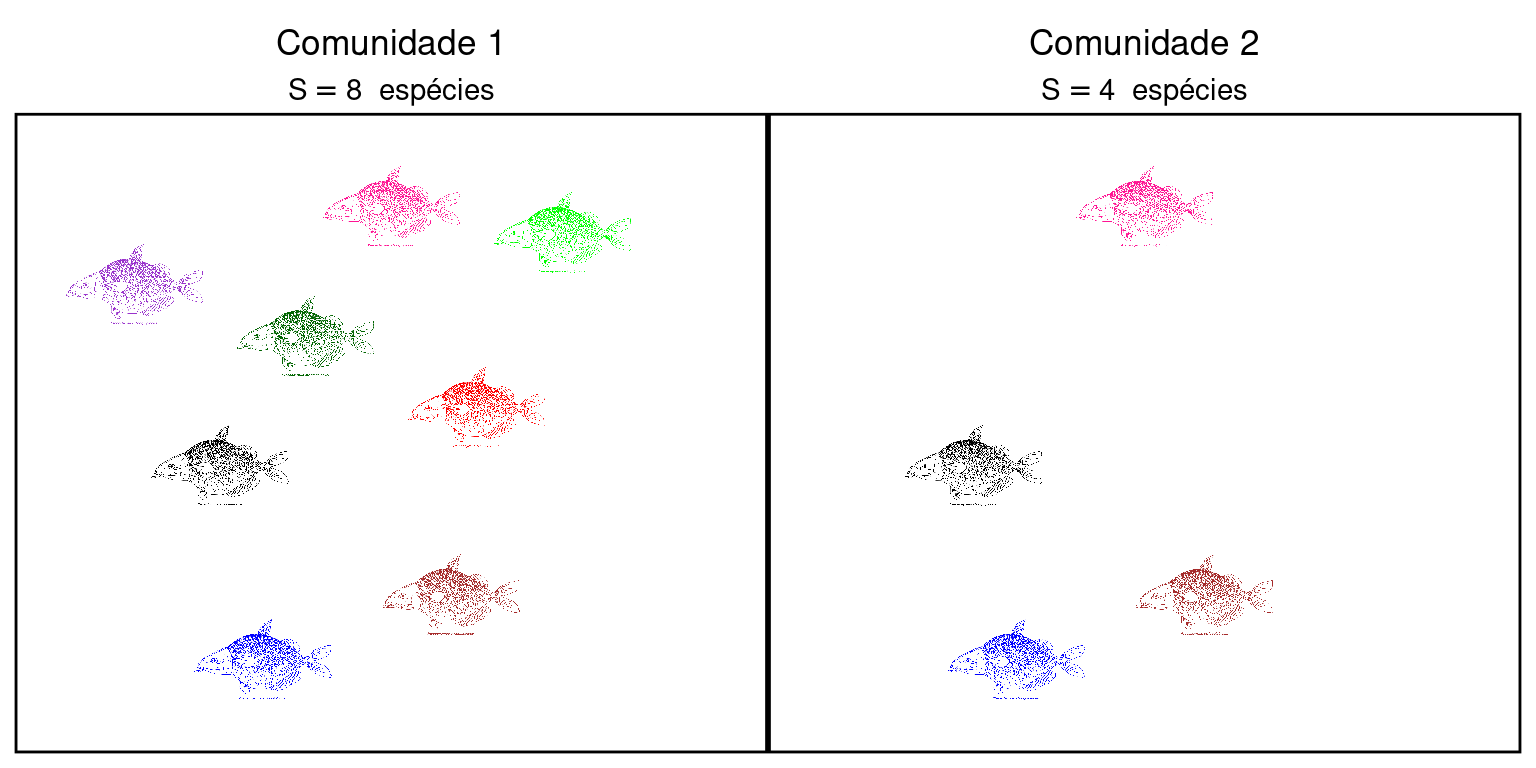
\includegraphics{medidas-diversidade_files/figure-latex/unnamed-chunk-4-1} \end{center}

Se medirmos a diversidade de uma comunidade por meio da riqueza de espécies, a comunidade \(1\) (\(S = 8\)) é duas vezes mais diversa que a comunidade \(2\) (\(S = 4\)). Entretanto, outro componente fundamental do que denominamos de diversidade de espécies tem relação com o \textbf{grau de uniformidade} ou \textbf{equabilidade} das abundâncias relativas. Se duas comunidades têm a mesma riqueza, será mais diversa aquela em que as abundâncias relativas forem mais uniformes entre as espécies.

Suponha duas comunidades com \(5\) espécies e \(100\) indivíduos. Na comunidade A todas as espécies têm \(20\) indivíduos, enquanto na comunidade B, a espécie mais abundante tem \(96\) indivíduos e todas as restantes somente \(1\) indivíduo cada. A comunidade A será mais diversa pois tem uma distribuição de abundância relativa mais uniforme, enquanto a segunda comunidade é menos uniforme (menos diversa) pois apresenta elevada \textbf{dominância}.

Ao combinarmos estes dois componentes podemos encontrar diferentes tipos de comunidades: i - comunidades com baixa riqueza de espécies e baixa dominância, ii - comunidades com baixa riqueza de espécies e alta dominância; iii - comunidades com alta riqueza de espécies e baixa dominância ou iii - comunidades com alta riqueza de espécies e alta dominância.

\begin{center}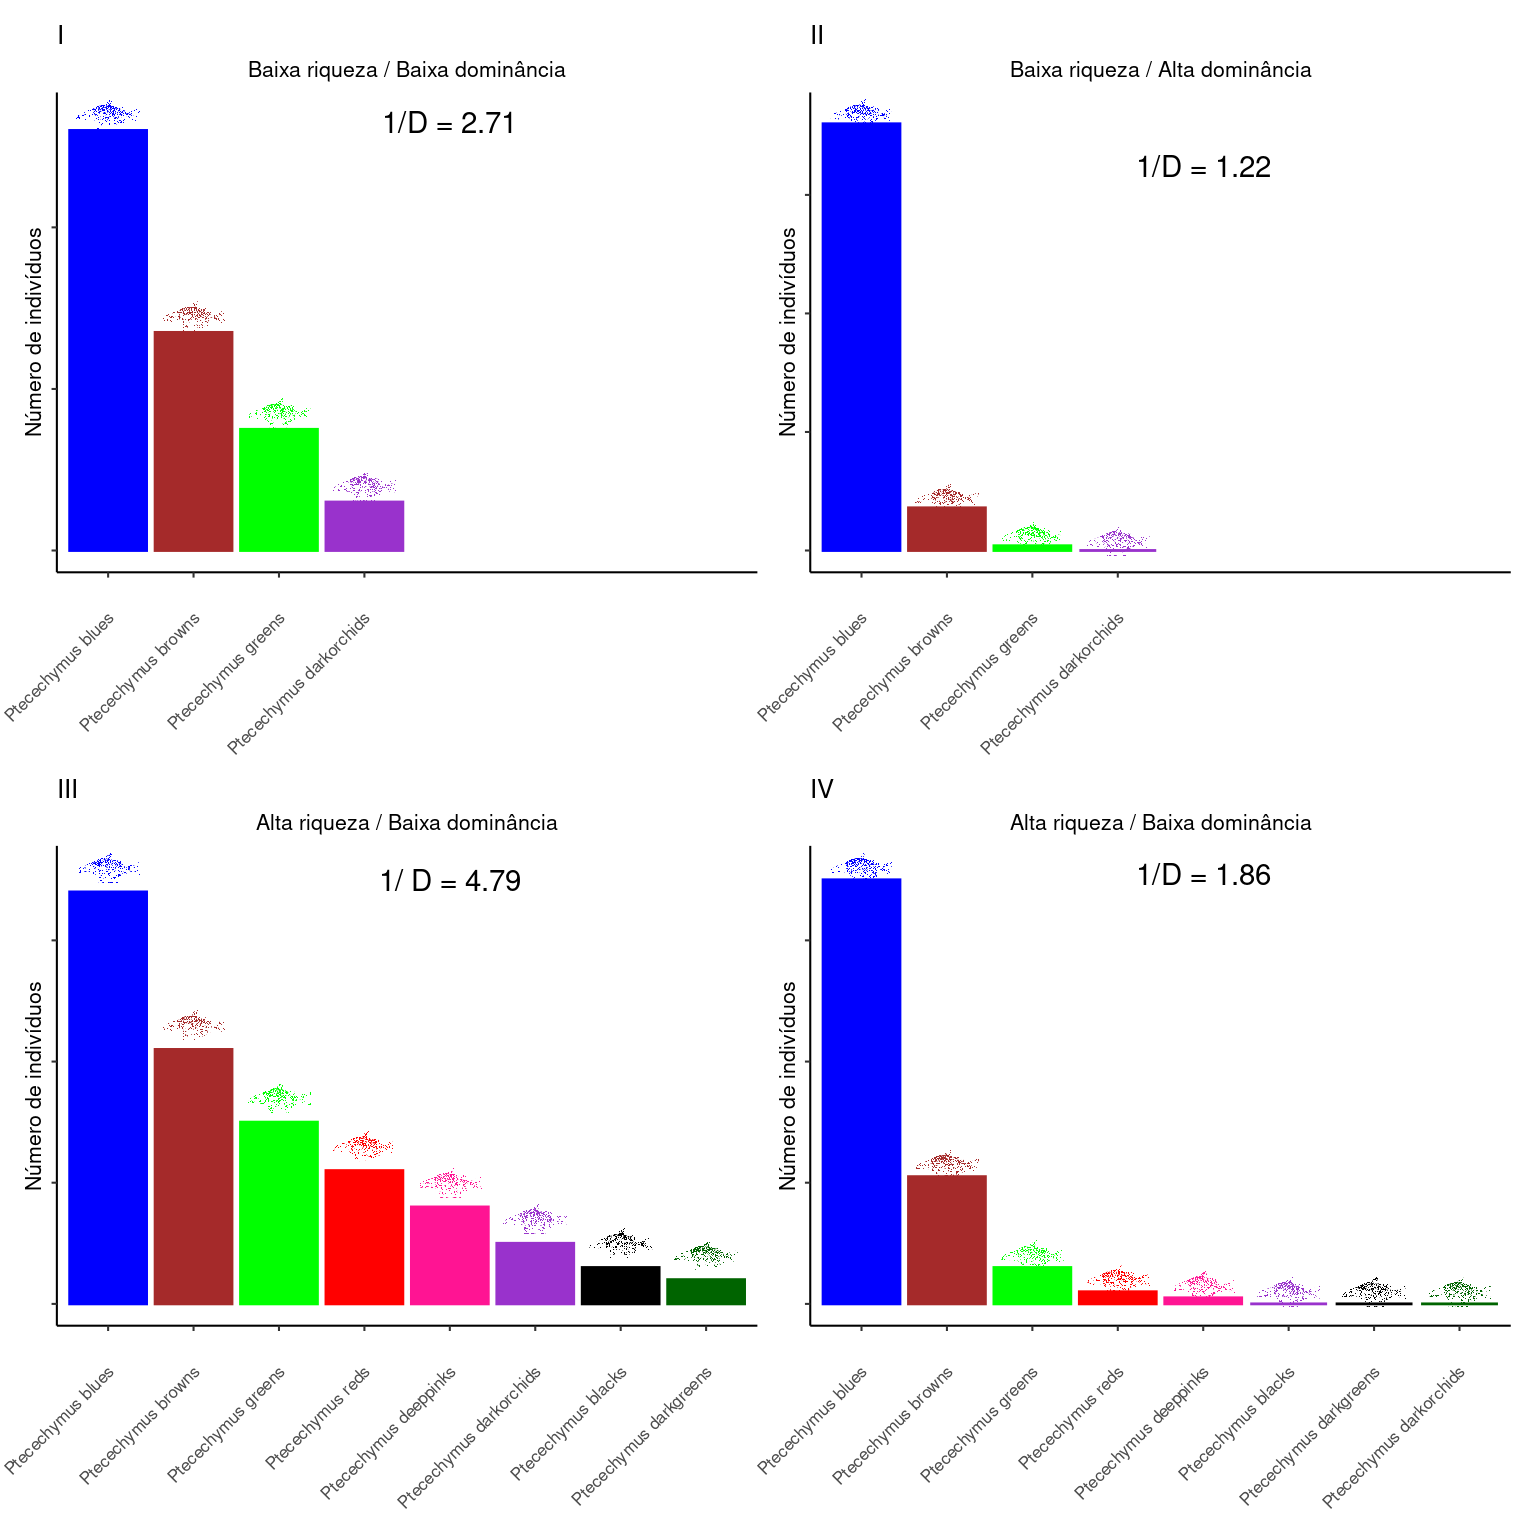
\includegraphics{medidas-diversidade_files/figure-latex/unnamed-chunk-7-1} \end{center}

\hypertarget{indices-de-diversidade}{%
\section{Indices de diversidade}\label{indices-de-diversidade}}

Os índices de diversidade capturam os dois componentes (riqueza de espécies e uniformidade) em uma única medida. Neste sentido, um elevado valor de diversidade pode ocorrer devido à elevada riqueza, elevada uniformidade (= baixa dominância), ou ambas.

Existe uma variedades de índices na literatura, cada um enfatizando em maior gau diferentes componentes (riqueza \emph{vs} equabilidade) da diversidade de espécies. Abaixo, vamos apresentar um deles, com propriedades bem conhecidas: o \textbf{Índice de Diversidade de Simpson}.

\textbf{Índice de Diversidade de Simpson}

Simpson (1949 - Measurement of diversity) definiu uma medida de diversidade a partir da probabilidade de que dois indivíduos retirados aleatoriamente de uma comunidade fossem pertencentes à mesma espécie. Para uma comunidade com número finito de indivíduos esta probabilidade pode ser dada por:

\[D = \sum_{i = 1}^{S}\left(\frac{n_i(n_1 - 1)}{N(N-1)}\right)\]

Se existe uma alta dominância, é \textbf{altamente provavel} que dois indivíduos retirados ao acaso sejam da mesma espécie. Deste modo, \(D\) dimuniu quando a comunidade é muito diversa. Para resolver esta questão o índice é comumente representado por seu inverso (\(1 - D\)) ou sua recíproca (\(1/D\)). O índice de Simpson captura a variância na distribuição de abundância das espécies, sobretudo para valores de riqueza acima de \(10\) (Maguran, 2004).

Para as comunidades representadas na figura anterior temos:

\begin{itemize}
\item
  Comunidade I: \(1/D = 2.71\)
\item
  Comunidade II: \(1/D = 1.22\)
\item
  Comunidade III: \(1/D = 4.79\)
\item
  Comunidade IV: \(1/D = 1.86\)
\end{itemize}

A comunidade \(III\) é a mais diversa pois possui elevada riqueza e alta uniformidade, enquanto a comunidade \(II\) é a menos diversa pois possui menor riqueza e baixa uniformidade. Finalmente, as comunidades \(I\) e \(IV\) ficam no meio do caminho, pois possuem baixa riqueza mas alta uniformidade ou vice-versa.

\textbf{Índice de Equabilidade de Simpson}

Uma vez que \(D\) combina riqueza com uniformidade, poderíamos buscar uma medida que evidenciasse somente a última (uma vez que a riqueza é simples de se obter). Se utilizarmos a diversidade de Simpson, teríamos a medida de \textbf{equabilidade de Simpson} como:

\[E_{1/D} = \frac{1/D}{S}\]

\(E_{1/D}\) varia entre \(0\) e \(1\) e não é sensível á riqueza de espécies.

Existe uma variedade de índices de diversidade e equabilidade. Para uma apresentação detalhada veja \citet{magurran2011medindo}, e uma discussão da relação entre riqueza, diversidade e equabilidade veja \citet{melo2008ganhamos} (acesse aqui).

\hypertarget{diversidade-na-paisagem}{%
\section{Diversidade na paisagem}\label{diversidade-na-paisagem}}

Ao olharmos para uma paisagem perceberemos que invariavelmente há algum grau de variabilidade na estrutura ambiental, sendo possivel muitas vezes reconhecer \textbf{manchas de habitats}. Considere por exemplo riachos em uma bacia costeira típica do litoral de São Paulo. Podemos encontar trechos com estruturas de hábitats altamente variáveis em termos tipo de substrato (rochoso \emph{vs} arenoso), largura, velocidade de corrente, sombreamento, etc.

\begin{center}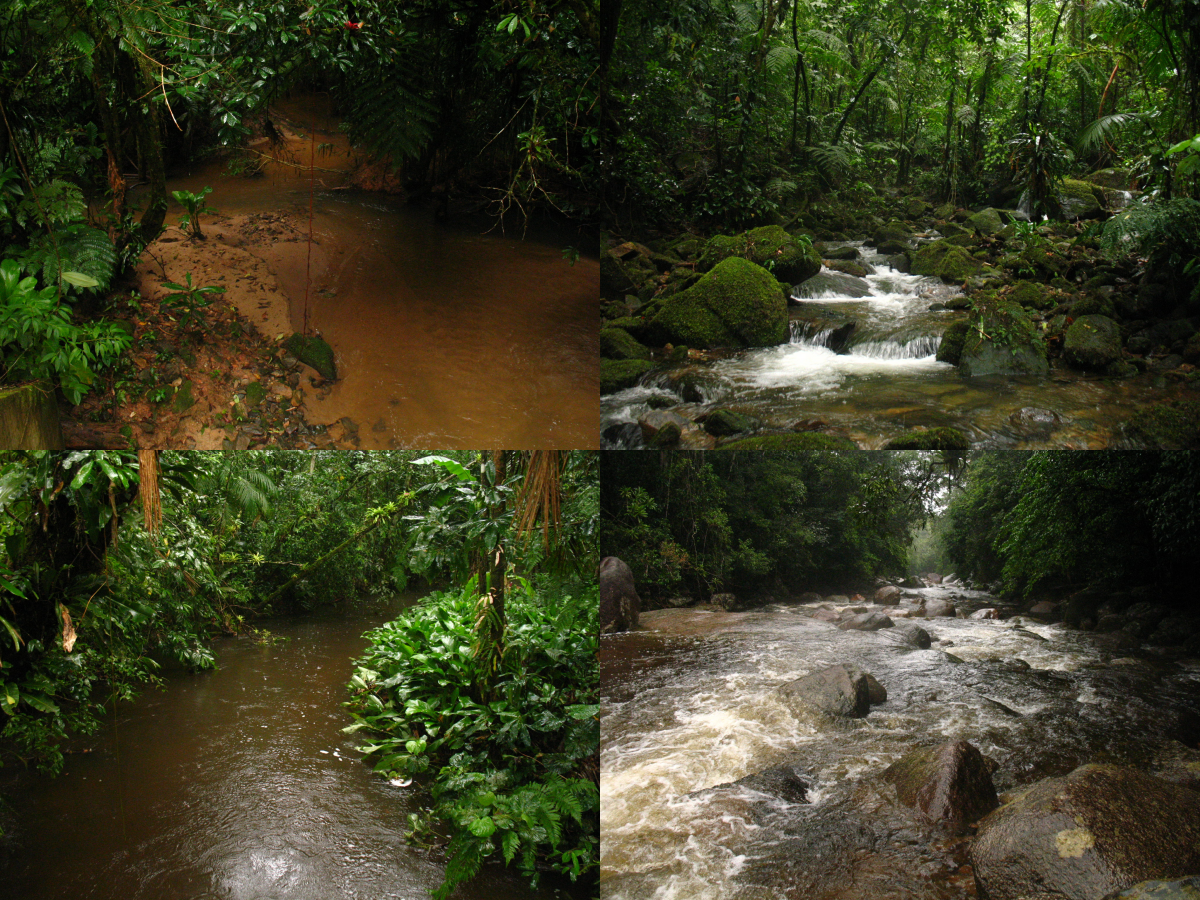
\includegraphics[width=16.67in]{medidas-diversidade_files/figure-latex/unnamed-chunk-8-1} \end{center}

É esperado que a composição de espécies presentes em cada um destes locais seja diferente, o que levará a variações nos padrões de riqueza e de equabilidade das comunidades. O mesmo vale para qualquer ambiente em que seja possível verificar alguma variação espacial na estrutura dos habitats. Algumas destas variações ocorrem em forma de gradiente ambiental. Por exemplo, há um gradiente de umidade e de exposição às ondas que vai do trecho superior (supral-itoral) ao trecho inferior (infra-litoral) de faixas de areia em praias. É esperado que a fauna que habite estes ambientes varie ao longo deste gradiente.

Mesmo que não haja um gradiente ambiental forte, ainda é esperado que devido à dinâmicas individuais de nascimento, morte, imigração, emigração, as espécies se distribuam de forma heterogênea na paisagem. Portanto, se queremos caracterizar a diveridade em uma determinada região, devemos amostrar diferentes parcelas na paisagem, o que nos leva a buscar padrões de diversidade em diferentes escalas.

Se tivermos na paisagem \(5\) comunidades diferentes, cada um com \(5\) espécies sem nenhuma sobreposição, a diversidade da paisagem será maior (\(S = 25\)) que as diversidades locais (\(S = 5\)).

Se por outro lado todas as comunidades tiverem exatamente as mesmas espécies, ao combiná-las, ainda teremos \(S = 5\) espécies na paisagem.

Muitas vezes não é possivel amostrar um hábitat por completo (por exemplo, toda a faixa de areia), ou ainda pode não ser possível sequer reconhecer manchas de hábitas. Ainda assim, o protocolo de amostragem será composto por unidades amostrais que se combinam para formar a amostra completa.

Imagine a amostragem de peixes na zona de arrebentação de praia da Baía de Santos. Cada amostra consiste do arrasto ao longo de \(200\) m. Ainda que não seja possível reconhecer limites físcos entre as comunidades que habitam a zona de arrebentação, a ideia de que a diversidade na Baía de Santos será composta da combinação entre as comunidades provinientes de cada arrasto ainda continua válida.

\begin{center}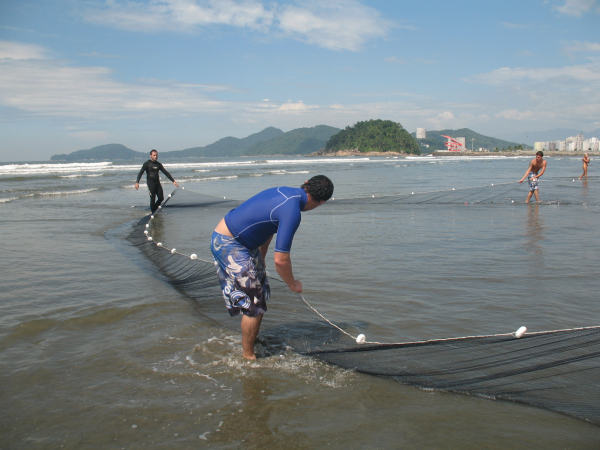
\includegraphics[width=8.33in]{medidas-diversidade_files/figure-latex/unnamed-chunk-9-1} \end{center}

Para organizar a diversidade em diferentes escalas, defini-se como diversidade \textbf{alfa (\(\alpha\))} a diversidade de uma única unidade amostral e como diversidade \textbf{gama (\(\gamma\))} a combinação de todas as diversidades locais na paisagem.

\begin{figure}

{\centering 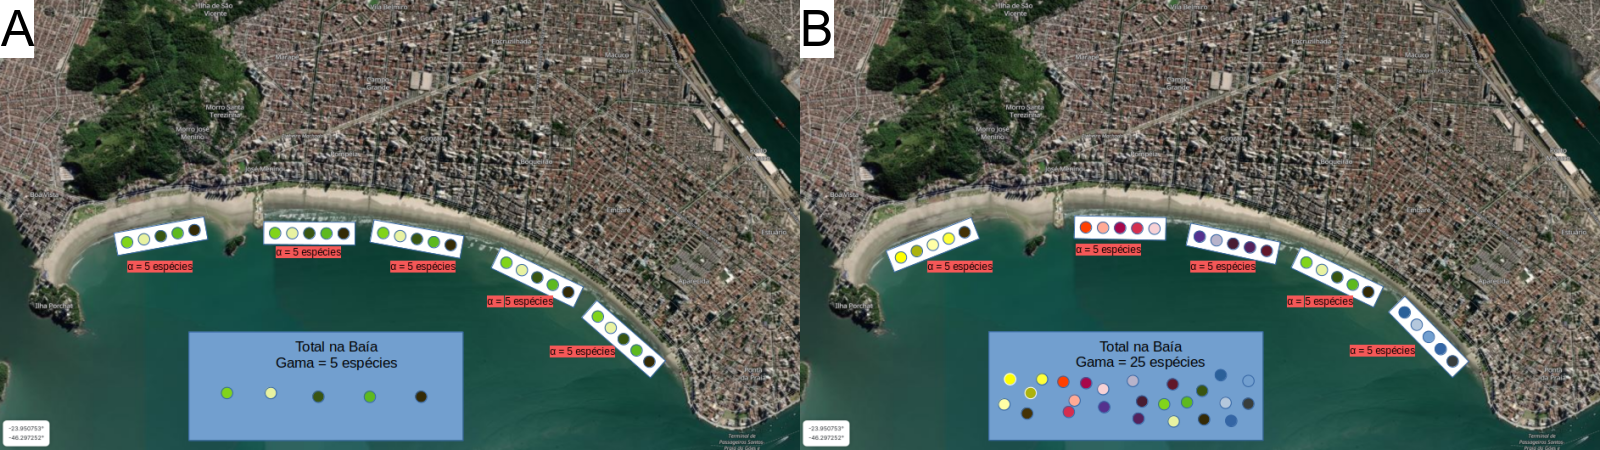
\includegraphics[width=16.67in]{medidas-diversidade_files/figure-latex/unnamed-chunk-10-1} 

}

\caption{A: Diversidade gama total (5 espécies) igual alfa locais (5 espécies). B: Diversidade gama total (25 espécies) maior alfa locais (5 espécies).}\label{fig:unnamed-chunk-10}
\end{figure}

Acima, temos na Figura 1.1A cinco amostras, cada uma contendo as mesmas \(5\) espécies. Ao combinarmos todas as amostras ainda teremos as mesmas espécies, de modo que as diversidades \(\alpha = \gamma = 5\) espécies.

Na Figura 1.1B também temos cinco amostras, porém cada uma contém \(5\) espécies totalmente diferentes das demais amostras. Neste caso, a diversidade na paisagem será \(\gamma = 25\) espécies, enquanto as diversidades locais conterão somente \(\alpha = 5\) espécies.

Para diferenciar situações destes tipo, definimos a \textbf{diversidade beta (\(\beta\))} que mede a diferença entre as diversidades \(\alpha\) e \(\gamma\). Nos exemplos acima temos que a Figura 1.1A descreve uma situação com \textbf{baixa diversidade \(\beta\)}, enquanto a Figura 1.1B descreve uma situação com \textbf{alta diversidade \(\beta\)}

No capítulo seguinte iremos descrever como podemos medir e compreender os padrões de diversidade de espécies nas diferentes escalas.

Para um texto introdutório sobre escalas de diversidade leia: Benone \& Montag (2021).

\hypertarget{diversidader}{%
\chapter{\texorpdfstring{Medindo as diversidades \(\alpha\), \(\beta\) e \(\gamma\): tutorial no R}{Medindo as diversidades \textbackslash alpha, \textbackslash beta e \textbackslash gamma: tutorial no R}}\label{diversidader}}

Neste tutorial iremos utilizar uma base de dados denominada Baia\_santos.xlsx, contendo a abundância de \(10\) espécies de peixes capturadas na zona de arrebentação da Baía de Santos em \(2015\). Cada linha da tabela representa uma amostra, isto é, um arrasto feito ao longo de \(200\) m na zona de arrebentação, seguindo a direção da linha da costa. No total foram \(12\) amostras. A primeira coluna identifica em que período do ano cada amostra foi obtida. As primeiras 6 foram tomadas no VERAO de \(2015\) e as outras 6 no INVERNO de \(2015\). As demais colunas mostram o número de indivíduos de cada espécie nas amostras. Os nomes das espécies foram omitidos para facilitar a apresentação dos dados.

Vamos utilizar esta tabela como exemplo para calcularmos as diversidades \(\alpha\), \(\beta\) e \(\gamma\).

\hypertarget{preparando-o-ambiente-de-trabalho}{%
\section{Preparando o ambiente de trabalho}\label{preparando-o-ambiente-de-trabalho}}

Os cálculos serão feitos no programa R. Antes de iniciar, é importante preparar seu ambiente de trabalho. Iremos utilizar o R-Studio como ambiente de programação, mas você pode utilizar outro editor de sua preferência. A seguir faremos toda a preparação necessária, mas pode ser útil consultar os links abaixo:

\begin{itemize}
\item
  Introdução ao Ambiente R de Programação - Capítulos 1 e 2
\item
  Estatística nas Ciências Ambientais - Capítulos 2 e 11
\end{itemize}

\begin{center}\rule{0.5\linewidth}{0.5pt}\end{center}

\begin{enumerate}
\def\labelenumi{\arabic{enumi}.}
\tightlist
\item
  Após abrir o R-Studio e criar um arquivo, direcione o R para o diretório onde você irá inserir seus dados. Por exemplo:
\end{enumerate}

\begin{Shaded}
\begin{Highlighting}[]
\FunctionTok{setwd}\NormalTok{(}\StringTok{\textquotesingle{}C:/Users/Usuario/Documents/Bio\_II\_2021\textquotesingle{}}\NormalTok{ )}
\end{Highlighting}
\end{Shaded}

\begin{enumerate}
\def\labelenumi{\arabic{enumi}.}
\setcounter{enumi}{1}
\item
  Faça o download da base de dados que iremos utilizar e salve dentro do diretório que você selecionou acima. O arquivo é do tipo \textbf{.xlsx} e está disponível para download no link Baia\_santos.xlsx
\item
  Caso ainda não tenha feito, instale os segintes pacotes com o comando abaixo:
\end{enumerate}

\begin{Shaded}
\begin{Highlighting}[]
\FunctionTok{install.packages}\NormalTok{(}\FunctionTok{c}\NormalTok{(}\StringTok{\textquotesingle{}readxl\textquotesingle{}}\NormalTok{, }\StringTok{\textquotesingle{}tidyverse\textquotesingle{}}\NormalTok{, }\StringTok{\textquotesingle{}vegan\textquotesingle{}}\NormalTok{, }\StringTok{\textquotesingle{}patchwork\textquotesingle{}}\NormalTok{, }\StringTok{\textquotesingle{}iNEXT\textquotesingle{}}\NormalTok{))}
\end{Highlighting}
\end{Shaded}

\begin{enumerate}
\def\labelenumi{\arabic{enumi}.}
\setcounter{enumi}{3}
\tightlist
\item
  Habilite os pacotes
\end{enumerate}

\begin{Shaded}
\begin{Highlighting}[]
\FunctionTok{library}\NormalTok{(readxl)}
\FunctionTok{library}\NormalTok{(tidyverse)}
\FunctionTok{library}\NormalTok{(vegan)}
\FunctionTok{library}\NormalTok{(patchwork)}
\FunctionTok{library}\NormalTok{(iNEXT)}
\end{Highlighting}
\end{Shaded}

\begin{quote}
Os pacotes precisam ser instalados somente uma vez. No entanto, sempre que você fechar e abrir o R-Studio, precisará habilitá-los novamente.
\end{quote}

\begin{enumerate}
\def\labelenumi{\arabic{enumi}.}
\setcounter{enumi}{4}
\tightlist
\item
  Importe a base de dados para o R-Studio
\end{enumerate}

\begin{Shaded}
\begin{Highlighting}[]
\NormalTok{pe }\OtherTok{=} \FunctionTok{read\_excel}\NormalTok{(}\StringTok{\textquotesingle{}Baia\_santos.xlsx\textquotesingle{}}\NormalTok{)}
\end{Highlighting}
\end{Shaded}

Após importar visualize a tabela:

\begin{Shaded}
\begin{Highlighting}[]
\FunctionTok{View}\NormalTok{(pe)}
\end{Highlighting}
\end{Shaded}

\begin{tabular}{l|r|r|r|r|r|r|r|r|r|r}
\hline
Epoca & sp\_1 & sp\_2 & sp\_3 & sp\_4 & sp\_5 & sp\_6 & sp\_7 & sp\_8 & sp\_9 & sp\_10\\
\hline
INVERNO & 5 & 6 & 72 & 65 & 8 & 6 & 1 & 0 & 0 & 0\\
\hline
INVERNO & 6 & 0 & 1 & 18 & 9 & 12 & 0 & 1 & 0 & 0\\
\hline
INVERNO & 7 & 0 & 0 & 48 & 2 & 0 & 0 & 4 & 0 & 0\\
\hline
INVERNO & 0 & 0 & 0 & 13 & 4 & 1 & 0 & 0 & 0 & 0\\
\hline
INVERNO & 2 & 0 & 143 & 48 & 1 & 0 & 0 & 1 & 0 & 0\\
\hline
INVERNO & 0 & 0 & 95 & 28 & 0 & 0 & 1 & 0 & 0 & 0\\
\hline
VERAO & 1 & 0 & 0 & 8 & 0 & 27 & 0 & 0 & 1 & 0\\
\hline
VERAO & 0 & 0 & 0 & 1 & 3 & 2 & 2 & 0 & 0 & 0\\
\hline
VERAO & 8 & 0 & 0 & 1 & 4 & 6 & 0 & 0 & 4 & 0\\
\hline
VERAO & 2 & 0 & 0 & 0 & 6 & 2 & 0 & 0 & 0 & 0\\
\hline
VERAO & 1 & 0 & 0 & 3 & 0 & 2 & 0 & 0 & 1 & 0\\
\hline
VERAO & 1 & 0 & 0 & 0 & 0 & 7 & 0 & 0 & 0 & 1\\
\hline
\end{tabular}

E verifique se as colunas foram lidas corretamente digitando o comando abaixo:

\begin{Shaded}
\begin{Highlighting}[]
\FunctionTok{glimpse}\NormalTok{(pe)}
\end{Highlighting}
\end{Shaded}

\begin{verbatim}
## Rows: 12
## Columns: 11
## $ Epoca <chr> "INVERNO", "INVERNO", "INVERNO", "INVERNO", "INVERNO", "INVERNO"~
## $ sp_1  <dbl> 5, 6, 7, 0, 2, 0, 1, 0, 8, 2, 1, 1
## $ sp_2  <dbl> 6, 0, 0, 0, 0, 0, 0, 0, 0, 0, 0, 0
## $ sp_3  <dbl> 72, 1, 0, 0, 143, 95, 0, 0, 0, 0, 0, 0
## $ sp_4  <dbl> 65, 18, 48, 13, 48, 28, 8, 1, 1, 0, 3, 0
## $ sp_5  <dbl> 8, 9, 2, 4, 1, 0, 0, 3, 4, 6, 0, 0
## $ sp_6  <dbl> 6, 12, 0, 1, 0, 0, 27, 2, 6, 2, 2, 7
## $ sp_7  <dbl> 1, 0, 0, 0, 0, 1, 0, 2, 0, 0, 0, 0
## $ sp_8  <dbl> 0, 1, 4, 0, 1, 0, 0, 0, 0, 0, 0, 0
## $ sp_9  <dbl> 0, 0, 0, 0, 0, 0, 1, 0, 4, 0, 1, 0
## $ sp_10 <dbl> 0, 0, 0, 0, 0, 0, 0, 0, 0, 0, 0, 1
\end{verbatim}

Você deve ver uma saída parecida com esta. Verifique se \texttt{Epoca} aparece com o símbolo \texttt{\textless{}chr\textgreater{}}, indicando que é uma variável categórica e se todas as demais aparecem com o símbolo \texttt{\textless{}dbl\textgreater{}}, indicando que são variáveis quantitativas. Caso alguma variável (exceto \texttt{Epoca}) apareça como \texttt{\textless{}chr\textgreater{}} você deve verificar em sua base de dados se existe algum caracter não numérico nas colunas das espécies.

\hypertarget{diversidade-alpha}{%
\section{\texorpdfstring{Diversidade \(\alpha\)}{Diversidade \textbackslash alpha}}\label{diversidade-alpha}}

A diversidade \(\alpha\) se refere às diversidades registradas localente, isto é, em cada uma das amostras. Após obtermos estas medidas, nos interessa entender qual é a diversidade média. Como dissemos no capítulo anterior, a diversidade pode ser caracterizada pela \textbf{riqueza de espécies}, \textbf{equabilidade} (ou uniformidade) ou um \textbf{índice de diversidade}. A riqueza refere-se simplesmente ao número de espécies em uma amostra. Se contarmos o número de espécies presentes na primeira linha da tabela por exemplo, encontraremos \(7\) espécies (sp\_1, sp\_2, sp\_3, sp\_4, sp\_5, sp\_6, sp\_7). Já na última amostra encontramos somente \(3\) espécies (sp\_1, sp\_6, sp\_10).

A equabilidade se refere ao padrão de distribuição das abundâncias relativas. Se todas as espécies forem \emph{igualmente} abundantes, a equabilidade é máxima. Por outro lado, se uma ou poucas espécies são muito abundantes e todas as demais raras (compostas por poucos indivíduos), a uniformidade é baixa (= dominância alta). Na linha \(3\) por exemplo, uma das espécies é composta por \(48\) individuos, enquanto a segunda espécie mais abundante apareceu com somente \(7\). Esta amostra possui elevada dominância.

Finalmente, os índices de diversidade combinam a riqueza de espécies e a equabilidade para nos fonecer uma medida-resumo para as comunidades locais.

Como temos amostras tomadas em dois períodos nos interessa comparar estes períodos em função das medidas de diversidade nas diferentes escalas.

\begin{tabular}{l|r|r|r|r|r|r|r|r|r|r}
\hline
Epoca & sp\_1 & sp\_2 & sp\_3 & sp\_4 & sp\_5 & sp\_6 & sp\_7 & sp\_8 & sp\_9 & sp\_10\\
\hline
\cellcolor[HTML]{7be896}{\textcolor{black}{INVERNO}} & \cellcolor[HTML]{7be896}{\textcolor{black}{5}} & \cellcolor[HTML]{7be896}{\textcolor{black}{6}} & \cellcolor[HTML]{7be896}{\textcolor{black}{72}} & \cellcolor[HTML]{7be896}{\textcolor{black}{65}} & \cellcolor[HTML]{7be896}{\textcolor{black}{8}} & \cellcolor[HTML]{7be896}{\textcolor{black}{6}} & \cellcolor[HTML]{7be896}{\textcolor{black}{1}} & \cellcolor[HTML]{7be896}{\textcolor{black}{0}} & \cellcolor[HTML]{7be896}{\textcolor{black}{0}} & \cellcolor[HTML]{7be896}{\textcolor{black}{0}}\\
\hline
\cellcolor[HTML]{7be896}{\textcolor{black}{INVERNO}} & \cellcolor[HTML]{7be896}{\textcolor{black}{6}} & \cellcolor[HTML]{7be896}{\textcolor{black}{0}} & \cellcolor[HTML]{7be896}{\textcolor{black}{1}} & \cellcolor[HTML]{7be896}{\textcolor{black}{18}} & \cellcolor[HTML]{7be896}{\textcolor{black}{9}} & \cellcolor[HTML]{7be896}{\textcolor{black}{12}} & \cellcolor[HTML]{7be896}{\textcolor{black}{0}} & \cellcolor[HTML]{7be896}{\textcolor{black}{1}} & \cellcolor[HTML]{7be896}{\textcolor{black}{0}} & \cellcolor[HTML]{7be896}{\textcolor{black}{0}}\\
\hline
\cellcolor[HTML]{7be896}{\textcolor{black}{INVERNO}} & \cellcolor[HTML]{7be896}{\textcolor{black}{7}} & \cellcolor[HTML]{7be896}{\textcolor{black}{0}} & \cellcolor[HTML]{7be896}{\textcolor{black}{0}} & \cellcolor[HTML]{7be896}{\textcolor{black}{48}} & \cellcolor[HTML]{7be896}{\textcolor{black}{2}} & \cellcolor[HTML]{7be896}{\textcolor{black}{0}} & \cellcolor[HTML]{7be896}{\textcolor{black}{0}} & \cellcolor[HTML]{7be896}{\textcolor{black}{4}} & \cellcolor[HTML]{7be896}{\textcolor{black}{0}} & \cellcolor[HTML]{7be896}{\textcolor{black}{0}}\\
\hline
\cellcolor[HTML]{7be896}{\textcolor{black}{INVERNO}} & \cellcolor[HTML]{7be896}{\textcolor{black}{0}} & \cellcolor[HTML]{7be896}{\textcolor{black}{0}} & \cellcolor[HTML]{7be896}{\textcolor{black}{0}} & \cellcolor[HTML]{7be896}{\textcolor{black}{13}} & \cellcolor[HTML]{7be896}{\textcolor{black}{4}} & \cellcolor[HTML]{7be896}{\textcolor{black}{1}} & \cellcolor[HTML]{7be896}{\textcolor{black}{0}} & \cellcolor[HTML]{7be896}{\textcolor{black}{0}} & \cellcolor[HTML]{7be896}{\textcolor{black}{0}} & \cellcolor[HTML]{7be896}{\textcolor{black}{0}}\\
\hline
\cellcolor[HTML]{7be896}{\textcolor{black}{INVERNO}} & \cellcolor[HTML]{7be896}{\textcolor{black}{2}} & \cellcolor[HTML]{7be896}{\textcolor{black}{0}} & \cellcolor[HTML]{7be896}{\textcolor{black}{143}} & \cellcolor[HTML]{7be896}{\textcolor{black}{48}} & \cellcolor[HTML]{7be896}{\textcolor{black}{1}} & \cellcolor[HTML]{7be896}{\textcolor{black}{0}} & \cellcolor[HTML]{7be896}{\textcolor{black}{0}} & \cellcolor[HTML]{7be896}{\textcolor{black}{1}} & \cellcolor[HTML]{7be896}{\textcolor{black}{0}} & \cellcolor[HTML]{7be896}{\textcolor{black}{0}}\\
\hline
\cellcolor[HTML]{7be896}{\textcolor{black}{INVERNO}} & \cellcolor[HTML]{7be896}{\textcolor{black}{0}} & \cellcolor[HTML]{7be896}{\textcolor{black}{0}} & \cellcolor[HTML]{7be896}{\textcolor{black}{95}} & \cellcolor[HTML]{7be896}{\textcolor{black}{28}} & \cellcolor[HTML]{7be896}{\textcolor{black}{0}} & \cellcolor[HTML]{7be896}{\textcolor{black}{0}} & \cellcolor[HTML]{7be896}{\textcolor{black}{1}} & \cellcolor[HTML]{7be896}{\textcolor{black}{0}} & \cellcolor[HTML]{7be896}{\textcolor{black}{0}} & \cellcolor[HTML]{7be896}{\textcolor{black}{0}}\\
\hline
\cellcolor[HTML]{e8867b}{\textcolor{black}{VERAO}} & \cellcolor[HTML]{e8867b}{\textcolor{black}{1}} & \cellcolor[HTML]{e8867b}{\textcolor{black}{0}} & \cellcolor[HTML]{e8867b}{\textcolor{black}{0}} & \cellcolor[HTML]{e8867b}{\textcolor{black}{8}} & \cellcolor[HTML]{e8867b}{\textcolor{black}{0}} & \cellcolor[HTML]{e8867b}{\textcolor{black}{27}} & \cellcolor[HTML]{e8867b}{\textcolor{black}{0}} & \cellcolor[HTML]{e8867b}{\textcolor{black}{0}} & \cellcolor[HTML]{e8867b}{\textcolor{black}{1}} & \cellcolor[HTML]{e8867b}{\textcolor{black}{0}}\\
\hline
\cellcolor[HTML]{e8867b}{\textcolor{black}{VERAO}} & \cellcolor[HTML]{e8867b}{\textcolor{black}{0}} & \cellcolor[HTML]{e8867b}{\textcolor{black}{0}} & \cellcolor[HTML]{e8867b}{\textcolor{black}{0}} & \cellcolor[HTML]{e8867b}{\textcolor{black}{1}} & \cellcolor[HTML]{e8867b}{\textcolor{black}{3}} & \cellcolor[HTML]{e8867b}{\textcolor{black}{2}} & \cellcolor[HTML]{e8867b}{\textcolor{black}{2}} & \cellcolor[HTML]{e8867b}{\textcolor{black}{0}} & \cellcolor[HTML]{e8867b}{\textcolor{black}{0}} & \cellcolor[HTML]{e8867b}{\textcolor{black}{0}}\\
\hline
\cellcolor[HTML]{e8867b}{\textcolor{black}{VERAO}} & \cellcolor[HTML]{e8867b}{\textcolor{black}{8}} & \cellcolor[HTML]{e8867b}{\textcolor{black}{0}} & \cellcolor[HTML]{e8867b}{\textcolor{black}{0}} & \cellcolor[HTML]{e8867b}{\textcolor{black}{1}} & \cellcolor[HTML]{e8867b}{\textcolor{black}{4}} & \cellcolor[HTML]{e8867b}{\textcolor{black}{6}} & \cellcolor[HTML]{e8867b}{\textcolor{black}{0}} & \cellcolor[HTML]{e8867b}{\textcolor{black}{0}} & \cellcolor[HTML]{e8867b}{\textcolor{black}{4}} & \cellcolor[HTML]{e8867b}{\textcolor{black}{0}}\\
\hline
\cellcolor[HTML]{e8867b}{\textcolor{black}{VERAO}} & \cellcolor[HTML]{e8867b}{\textcolor{black}{2}} & \cellcolor[HTML]{e8867b}{\textcolor{black}{0}} & \cellcolor[HTML]{e8867b}{\textcolor{black}{0}} & \cellcolor[HTML]{e8867b}{\textcolor{black}{0}} & \cellcolor[HTML]{e8867b}{\textcolor{black}{6}} & \cellcolor[HTML]{e8867b}{\textcolor{black}{2}} & \cellcolor[HTML]{e8867b}{\textcolor{black}{0}} & \cellcolor[HTML]{e8867b}{\textcolor{black}{0}} & \cellcolor[HTML]{e8867b}{\textcolor{black}{0}} & \cellcolor[HTML]{e8867b}{\textcolor{black}{0}}\\
\hline
\cellcolor[HTML]{e8867b}{\textcolor{black}{VERAO}} & \cellcolor[HTML]{e8867b}{\textcolor{black}{1}} & \cellcolor[HTML]{e8867b}{\textcolor{black}{0}} & \cellcolor[HTML]{e8867b}{\textcolor{black}{0}} & \cellcolor[HTML]{e8867b}{\textcolor{black}{3}} & \cellcolor[HTML]{e8867b}{\textcolor{black}{0}} & \cellcolor[HTML]{e8867b}{\textcolor{black}{2}} & \cellcolor[HTML]{e8867b}{\textcolor{black}{0}} & \cellcolor[HTML]{e8867b}{\textcolor{black}{0}} & \cellcolor[HTML]{e8867b}{\textcolor{black}{1}} & \cellcolor[HTML]{e8867b}{\textcolor{black}{0}}\\
\hline
\cellcolor[HTML]{e8867b}{\textcolor{black}{VERAO}} & \cellcolor[HTML]{e8867b}{\textcolor{black}{1}} & \cellcolor[HTML]{e8867b}{\textcolor{black}{0}} & \cellcolor[HTML]{e8867b}{\textcolor{black}{0}} & \cellcolor[HTML]{e8867b}{\textcolor{black}{0}} & \cellcolor[HTML]{e8867b}{\textcolor{black}{0}} & \cellcolor[HTML]{e8867b}{\textcolor{black}{7}} & \cellcolor[HTML]{e8867b}{\textcolor{black}{0}} & \cellcolor[HTML]{e8867b}{\textcolor{black}{0}} & \cellcolor[HTML]{e8867b}{\textcolor{black}{0}} & \cellcolor[HTML]{e8867b}{\textcolor{black}{1}}\\
\hline
\end{tabular}

Vamos adicionar ao final da tabela \texttt{pe} três colunas, uma com a riqueza de espécies (\(S\)), uma com o índice de diversidade de Simpson (\(D\)) e outra com a equabilidade de Simpson (\(E\)). Desta forma teremos as três medidas de diversidade relevantes em nossa discussão.

\begin{Shaded}
\begin{Highlighting}[]
\NormalTok{pe }\OtherTok{=}\NormalTok{ pe }\SpecialCharTok{\%\textgreater{}\%}
  \FunctionTok{rowwise}\NormalTok{() }\SpecialCharTok{\%\textgreater{}\%} 
  \FunctionTok{mutate}\NormalTok{(}\AttributeTok{S =} \FunctionTok{specnumber}\NormalTok{(}\FunctionTok{c\_across}\NormalTok{(sp\_1}\SpecialCharTok{:}\NormalTok{sp\_10)),}
         \AttributeTok{D =} \FunctionTok{diversity}\NormalTok{(}\FunctionTok{c\_across}\NormalTok{(sp\_1}\SpecialCharTok{:}\NormalTok{sp\_10), }
                       \AttributeTok{index =} \StringTok{\textquotesingle{}invsimpson\textquotesingle{}}\NormalTok{)) }\SpecialCharTok{\%\textgreater{}\%} 
  \FunctionTok{mutate}\NormalTok{(}\AttributeTok{E =}\NormalTok{ D}\SpecialCharTok{/}\NormalTok{S)}
\end{Highlighting}
\end{Shaded}

Ao digitar a tabela novamente veremos as três novas colunas, mostrando que para cada amostra foi calculado um valor de \(S\), \(D\) e \(E\).

\begin{Shaded}
\begin{Highlighting}[]
\FunctionTok{View}\NormalTok{(pe)}
\end{Highlighting}
\end{Shaded}

\begin{table}
\centering\begingroup\fontsize{10}{12}\selectfont

\begin{tabular}{l|r|r|r|r|r|r|r|r|r|r|r|r|r}
\hline
Epoca & sp\_1 & sp\_2 & sp\_3 & sp\_4 & sp\_5 & sp\_6 & sp\_7 & sp\_8 & sp\_9 & sp\_10 & S & D & E\\
\hline
INVERNO & 5 & 6 & 72 & 65 & 8 & 6 & 1 & 0 & 0 & 0 & 7 & 2.775990 & 0.3965700\\
\hline
INVERNO & 6 & 0 & 1 & 18 & 9 & 12 & 0 & 1 & 0 & 0 & 6 & 3.763203 & 0.6272005\\
\hline
INVERNO & 7 & 0 & 0 & 48 & 2 & 0 & 0 & 4 & 0 & 0 & 4 & 1.568057 & 0.3920143\\
\hline
INVERNO & 0 & 0 & 0 & 13 & 4 & 1 & 0 & 0 & 0 & 0 & 3 & 1.741936 & 0.5806452\\
\hline
INVERNO & 2 & 0 & 143 & 48 & 1 & 0 & 0 & 1 & 0 & 0 & 5 & 1.670768 & 0.3341535\\
\hline
INVERNO & 0 & 0 & 95 & 28 & 0 & 0 & 1 & 0 & 0 & 0 & 3 & 1.567380 & 0.5224601\\
\hline
VERAO & 1 & 0 & 0 & 8 & 0 & 27 & 0 & 0 & 1 & 0 & 4 & 1.722013 & 0.4305031\\
\hline
VERAO & 0 & 0 & 0 & 1 & 3 & 2 & 2 & 0 & 0 & 0 & 4 & 3.555556 & 0.8888889\\
\hline
VERAO & 8 & 0 & 0 & 1 & 4 & 6 & 0 & 0 & 4 & 0 & 5 & 3.977444 & 0.7954887\\
\hline
VERAO & 2 & 0 & 0 & 0 & 6 & 2 & 0 & 0 & 0 & 0 & 3 & 2.272727 & 0.7575758\\
\hline
VERAO & 1 & 0 & 0 & 3 & 0 & 2 & 0 & 0 & 1 & 0 & 4 & 3.266667 & 0.8166667\\
\hline
VERAO & 1 & 0 & 0 & 0 & 0 & 7 & 0 & 0 & 0 & 1 & 3 & 1.588235 & 0.5294118\\
\hline
\end{tabular}
\endgroup{}
\end{table}

\begin{quote}
Para manter a notação simples, estamos utilizando a simbologia \(D\) mas, extritamente falando, o argumento \texttt{index\ =\ \textquotesingle{}invsimpson\textquotesingle{}} calcula a recíproca do índice de Simpson (\(1/D\)). Deste modo valores mais altos são associados à comunidades mais diversas.
\end{quote}

Para compararmos a diversidade \(\alpha\) entre os períodos de VERAO e INVERNO vamos fazer um \texttt{boxplot} e sobrepor um gráfico de dispersão.

\begin{Shaded}
\begin{Highlighting}[]
\NormalTok{plt\_D }\OtherTok{=} \FunctionTok{ggplot}\NormalTok{(pe) }\SpecialCharTok{+}
  \FunctionTok{aes}\NormalTok{(}\AttributeTok{x =}\NormalTok{ Epoca, }\AttributeTok{y =}\NormalTok{ D) }\SpecialCharTok{+}
  \FunctionTok{geom\_boxplot}\NormalTok{(}\AttributeTok{fill =} \StringTok{\textquotesingle{}lightblue\textquotesingle{}}\NormalTok{, }\AttributeTok{alpha =} \FloatTok{0.5}\NormalTok{) }\SpecialCharTok{+}
  \FunctionTok{geom\_jitter}\NormalTok{(}\AttributeTok{width =} \FloatTok{0.1}\NormalTok{, }\AttributeTok{size =} \DecValTok{3}\NormalTok{) }\SpecialCharTok{+}
  \FunctionTok{labs}\NormalTok{(}\AttributeTok{y =} \StringTok{\textquotesingle{}Diversidade de Simpson (1/D)\textquotesingle{}}\NormalTok{, }
        \AttributeTok{x =} \StringTok{\textquotesingle{}\textquotesingle{}}\NormalTok{) }\SpecialCharTok{+}
  \FunctionTok{theme\_classic}\NormalTok{()}

\NormalTok{plt\_S }\OtherTok{=} \FunctionTok{ggplot}\NormalTok{(pe) }\SpecialCharTok{+}
  \FunctionTok{aes}\NormalTok{(}\AttributeTok{x =}\NormalTok{ Epoca, }\AttributeTok{y =}\NormalTok{ S) }\SpecialCharTok{+}
  \FunctionTok{geom\_boxplot}\NormalTok{(}\AttributeTok{fill =} \StringTok{\textquotesingle{}lightblue\textquotesingle{}}\NormalTok{, }\AttributeTok{alpha =} \FloatTok{0.5}\NormalTok{) }\SpecialCharTok{+}
  \FunctionTok{geom\_jitter}\NormalTok{(}\AttributeTok{width =} \FloatTok{0.1}\NormalTok{, }\AttributeTok{size =} \DecValTok{3}\NormalTok{) }\SpecialCharTok{+}
  \FunctionTok{labs}\NormalTok{(}\AttributeTok{y =} \StringTok{\textquotesingle{}Riqueza de Espécies (S)\textquotesingle{}}\NormalTok{, }
        \AttributeTok{x =} \StringTok{\textquotesingle{}\textquotesingle{}}\NormalTok{) }\SpecialCharTok{+}
  \FunctionTok{theme\_classic}\NormalTok{()}

\NormalTok{plt\_E }\OtherTok{=} \FunctionTok{ggplot}\NormalTok{(pe) }\SpecialCharTok{+}
  \FunctionTok{aes}\NormalTok{(}\AttributeTok{x =}\NormalTok{ Epoca, }\AttributeTok{y =}\NormalTok{ E) }\SpecialCharTok{+}
  \FunctionTok{geom\_boxplot}\NormalTok{(}\AttributeTok{fill =} \StringTok{\textquotesingle{}lightblue\textquotesingle{}}\NormalTok{, }\AttributeTok{alpha =} \FloatTok{0.5}\NormalTok{) }\SpecialCharTok{+}
  \FunctionTok{geom\_jitter}\NormalTok{(}\AttributeTok{width =} \FloatTok{0.1}\NormalTok{, }\AttributeTok{size =} \DecValTok{3}\NormalTok{) }\SpecialCharTok{+}
  \FunctionTok{labs}\NormalTok{(}\AttributeTok{y =} \StringTok{\textquotesingle{}Equabilidade de Simpson (E)\textquotesingle{}}\NormalTok{, }
        \AttributeTok{x =} \StringTok{\textquotesingle{}\textquotesingle{}}\NormalTok{) }\SpecialCharTok{+}
  \FunctionTok{theme\_classic}\NormalTok{()}
\end{Highlighting}
\end{Shaded}

\begin{Shaded}
\begin{Highlighting}[]
\NormalTok{plt\_D }\SpecialCharTok{|}\NormalTok{ plt\_S }\SpecialCharTok{|}\NormalTok{ plt\_E}
\end{Highlighting}
\end{Shaded}

\begin{center}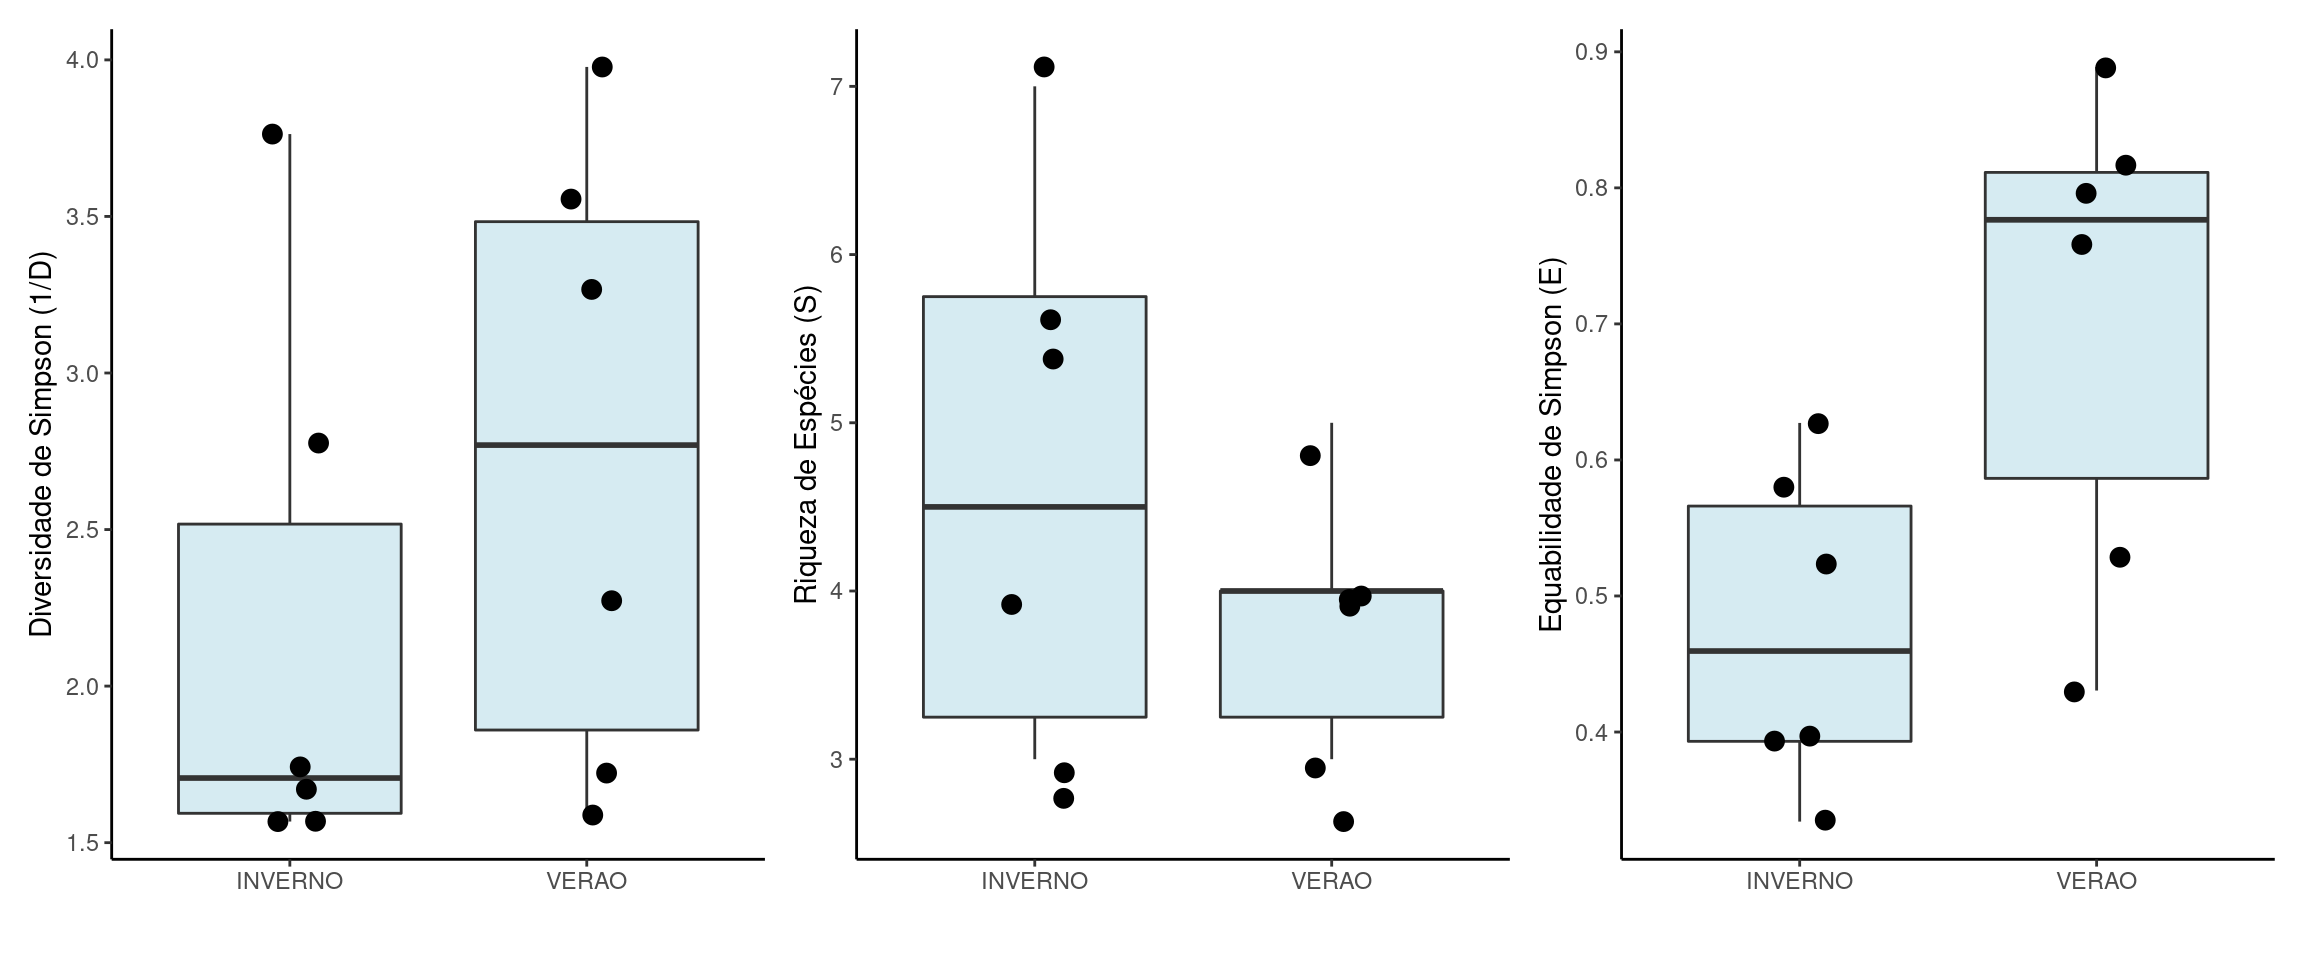
\includegraphics{medidas-diversidade_files/figure-latex/unnamed-chunk-26-1} \end{center}

\begin{quote}
Para visualizar os gráficos lado-a-lado com o comando acima, você deve ter instalado e habilitado o pacote \texttt{patchwork}.
\end{quote}

Nas figuras, a diversidade medida pelo índice de Simpson parace mais elevada no período do VERAO. Entretanto a riqueza parece menor neste período, sugerindo que a elevada diversidade foi observada principalmente por influência da equabilidade, claramente mais elevada no VERAO. Deste modo, embora no período do inverno tenham aparecido em média mais espécies, a dominânca também foi maior, fazendso com que a diversidade ficasse reduzida. Como a diversidade é sempre uma medida comparativa, é importante observar os três componentes da diversidade.

\begin{quote}
\emph{Para detalhes sobre a construção de um boxplot, veja o link:} Estatística nas Ciências Ambientais - Capítulos 7 e 11
\end{quote}

\hypertarget{diversidade-gamma}{%
\section{\texorpdfstring{Diversidade \(\gamma\)}{Diversidade \textbackslash gamma}}\label{diversidade-gamma}}

A princípio, a diversidade \(\gamma\) pode ser medida com qualquer um dos índices utilizados para descrever a diversidade \(\alpha\), bastando para isto somar as abundâncias das espécies em todos os pontos. Entretanto, quando olhamos para a diversidade total uma pergunta que devemos nos fazer é:

\begin{quote}
O número de amostras que tenho em mãos foi suficiente para caracterizar a comunidade?
\end{quote}

É esperado por exemplo que ao adicionamos novas amostras, a riqueza de espécies total aumente. Em nosso exemplo, se tivéssemos somente uma amostra, certamente não veríamos todas as \(10\) espécies de nossa matriz. Ao adicionar uma segunda amostra, podem surgir novas espécies não observadas na primeira, fazendo com que o número total aumente. À medida que continuamos adicionando amostras novas, é esperado que outras espécias vão sendo acumuladas no cômputo total. Entretanto, em algum momento é esperado que já tenhamos observado todas as espécies e a partir daí, a adição de novas amostras não trará nenhuma espécie que já não tenha sido observada. Neste momento, saberemos que a comunidade foi adequadamente caracterizada por sua riqueza total.

Para verificarmos como o número de espécies total aumenta com o número de amostras locais podemos construir uma \textbf{curva de acumulação de espécies} ou \textbf{curva do coletor}. Se fizermos isto para as seis amostras do VERAO teríamos:

\begin{Shaded}
\begin{Highlighting}[]
\NormalTok{ac\_verao }\OtherTok{=}\NormalTok{ pe }\SpecialCharTok{\%\textgreater{}\%} 
  \FunctionTok{filter}\NormalTok{(Epoca }\SpecialCharTok{==} \StringTok{\textquotesingle{}VERAO\textquotesingle{}}\NormalTok{) }\SpecialCharTok{\%\textgreater{}\%}
  \FunctionTok{select}\NormalTok{(sp\_1}\SpecialCharTok{:}\NormalTok{sp\_10) }\SpecialCharTok{\%\textgreater{}\%} 
  \FunctionTok{specaccum}\NormalTok{(}\AttributeTok{method =} \StringTok{\textquotesingle{}collector\textquotesingle{}}\NormalTok{)}

\FunctionTok{plot}\NormalTok{(}\AttributeTok{y =}\NormalTok{ ac\_verao}\SpecialCharTok{$}\NormalTok{richness, }\AttributeTok{x =}\NormalTok{ ac\_verao}\SpecialCharTok{$}\NormalTok{sites,}
     \AttributeTok{type =} \StringTok{\textquotesingle{}b\textquotesingle{}}\NormalTok{, }\AttributeTok{pch =} \DecValTok{19}\NormalTok{, }\AttributeTok{col =} \DecValTok{2}\NormalTok{, }\AttributeTok{lty =} \DecValTok{2}\NormalTok{,}
     \AttributeTok{ylab =} \StringTok{\textquotesingle{}Riqueza acumulada\textquotesingle{}}\NormalTok{,}
     \AttributeTok{xlab =} \StringTok{\textquotesingle{}Número de amostras\textquotesingle{}}\NormalTok{)}
\end{Highlighting}
\end{Shaded}

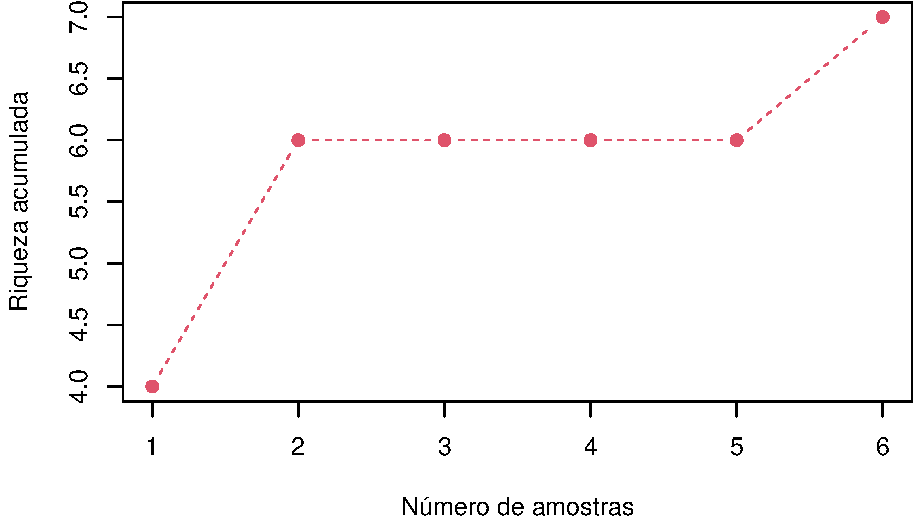
\includegraphics{medidas-diversidade_files/figure-latex/unnamed-chunk-27-1.pdf}

Esta figura mostra que na primeira amostra do verão foram observadas \(4\) espécies. Ao adicionar a segunda amostra, verificamos duas espécies adicionais, totalizando \(6\) espécies. Nenhuma espécie adicional foi observada da \(3^a\) a \(5^a\) amostra. Somente na \(6^a\) amostra, mais uma espécie foi observada, totalizando \(7\) espécies capturadas no período do VERAO.

A figura mostrada acima seguiu exatamente a sequência de amostras das linhas de nossa tabela. No entanto qualquer outra sequência seria igualmente válida. Assim, para termos um padrão \textbf{esperado}, existem vários métodos que nos permitirão encontrar uma valor de riqueza \textbf{médio} como função do número de amostras.

A mesma ideia pode ser reformulada pensando na adição de indivíduos, isto é: a partir de quantos indivíduos amostrados a comunidade terá sua riqueza adaquadamente caracterizada?

Vamos avalir esta questão para nossas comunidades de VERAO e de INVERNO, construindo curvas de acumulação para a riqueza de espécies como função do número de indivíduos nas amostras. Para isto, vamos utilizar o pacote iNEXT.

Inicialmente, precisamos criar uma lista separando as comunidades de verão e inverno:

\begin{Shaded}
\begin{Highlighting}[]
\NormalTok{pe\_list }\OtherTok{=} \FunctionTok{list}\NormalTok{()}
\NormalTok{pe\_list}\SpecialCharTok{$}\NormalTok{VERAO }\OtherTok{=}\NormalTok{ pe }\SpecialCharTok{\%\textgreater{}\%} 
  \FunctionTok{filter}\NormalTok{(Epoca }\SpecialCharTok{==} \StringTok{\textquotesingle{}VERAO\textquotesingle{}}\NormalTok{) }\SpecialCharTok{\%\textgreater{}\%} 
  \FunctionTok{select}\NormalTok{(sp\_1}\SpecialCharTok{:}\NormalTok{sp\_10) }\SpecialCharTok{\%\textgreater{}\%} 
  \FunctionTok{colSums}\NormalTok{()}
  
\NormalTok{pe\_list}\SpecialCharTok{$}\NormalTok{INVERNO }\OtherTok{=}\NormalTok{ pe }\SpecialCharTok{\%\textgreater{}\%} 
  \FunctionTok{filter}\NormalTok{(Epoca }\SpecialCharTok{==} \StringTok{\textquotesingle{}INVERNO\textquotesingle{}}\NormalTok{) }\SpecialCharTok{\%\textgreater{}\%} 
  \FunctionTok{select}\NormalTok{(sp\_1}\SpecialCharTok{:}\NormalTok{sp\_10) }\SpecialCharTok{\%\textgreater{}\%} 
  \FunctionTok{colSums}\NormalTok{()}
\end{Highlighting}
\end{Shaded}

Em seguida, utilizamos a função \texttt{iNEXT}, com os argumentos \texttt{datatype\ =\ \textquotesingle{}abundance\textquotesingle{}} (indivíduos no eixo \(x\)) e \texttt{q\ =\ 0} (riqueza acumulada no eixo \(y\)).

\begin{Shaded}
\begin{Highlighting}[]
\NormalTok{gama\_ac }\OtherTok{=} \FunctionTok{iNEXT}\NormalTok{(pe\_list, }
                 \AttributeTok{datatype =} \StringTok{\textquotesingle{}abundance\textquotesingle{}}\NormalTok{, }
                 \AttributeTok{q =} \DecValTok{0}\NormalTok{)}

\NormalTok{plt\_gama }\OtherTok{=} \FunctionTok{ggiNEXT}\NormalTok{(gama\_ac) }\SpecialCharTok{+}
  \FunctionTok{labs}\NormalTok{(}\AttributeTok{y =} \StringTok{\textquotesingle{}Riqueza acumulada\textquotesingle{}}\NormalTok{,}
       \AttributeTok{x =} \StringTok{\textquotesingle{}Número de indivíduos\textquotesingle{}}\NormalTok{) }\SpecialCharTok{+}
  \FunctionTok{theme\_classic}\NormalTok{() }\SpecialCharTok{+}
  \FunctionTok{scale\_y\_continuous}\NormalTok{(}\AttributeTok{breaks =} \DecValTok{0}\SpecialCharTok{:}\DecValTok{10}\NormalTok{) }\SpecialCharTok{+}
  \FunctionTok{theme}\NormalTok{(}\AttributeTok{legend.position =} \StringTok{"bottom"}\NormalTok{, }
        \AttributeTok{legend.title=}\FunctionTok{element\_blank}\NormalTok{())}
\end{Highlighting}
\end{Shaded}

As curvas de acumulo de espécies nos dois períodos ficam:

\begin{Shaded}
\begin{Highlighting}[]
\NormalTok{plt\_gama}
\end{Highlighting}
\end{Shaded}

\begin{center}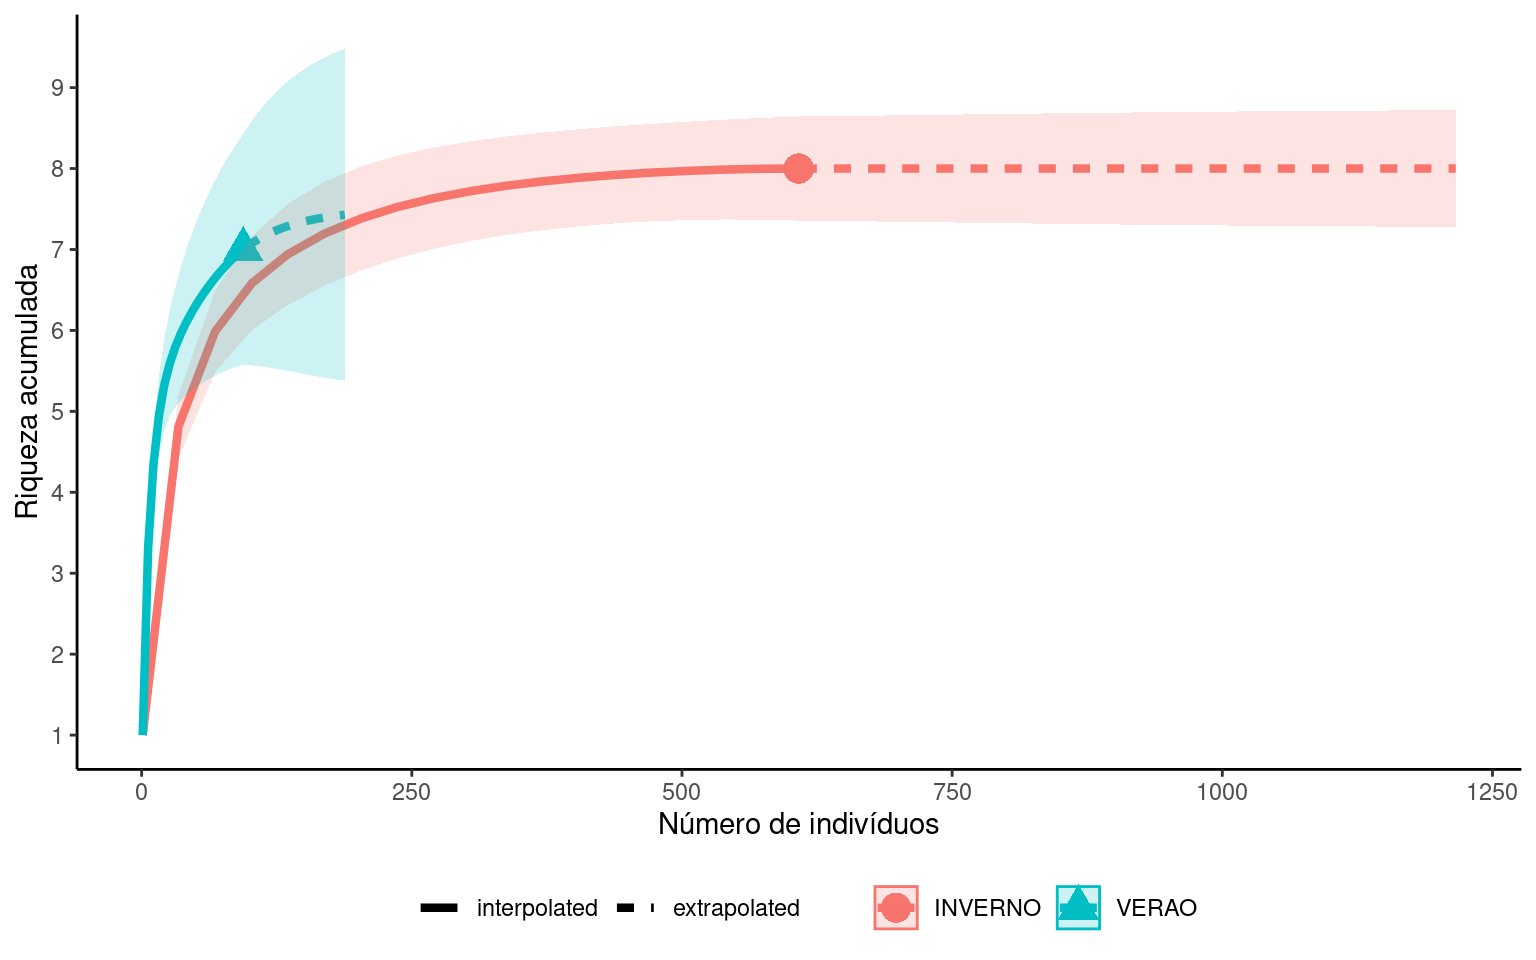
\includegraphics{medidas-diversidade_files/figure-latex/unnamed-chunk-30-1} \end{center}

As funções do pacote \texttt{iNEXT} nos permitem uma \textbf{extrapolação} do que seria esperado se continuássemos coletando. Desta figura percebemos dois pontos importantes.

\begin{itemize}
\item
  a riqueza total é similar entre os períodos, ainda que localmente, o verão tenha tido em média menores riqueza locais (veja padrões de diversidade \(\alpha\)).
\item
  A comunidade de INVERNO tem mais indivíduos e aparentemente foi melhor caracterizada, uma vez que a riqueza de espécies acumulada parece se estabilizar ao redor de 8 espécies. A comunidade de VERAO por outro lado, teve poucos indivíduos amostrados, de modo que ainda não há informação o suficiente para sabermos o que poderia acontecer caso continuássemos a amostrar as comunidades neste período. Esta incerteza pode ser observada na larga faixa em verde que contrasta com a faixa em vermelho mais estreita.
\end{itemize}

\hypertarget{diversidade-beta}{%
\section{\texorpdfstring{Diversidade \(\beta\)}{Diversidade \textbackslash beta}}\label{diversidade-beta}}

A diversidade \(\beta\) mede o grau de diferenciação entre manchas de habitat na paisagem. Tradicionalmente, duas abordagens têm sido utilizadas para expressar a diversidade \(\beta\). A primeira é baseada na comparação entre a diversidade \(\gamma\) da paisagem e as diversidades \(\alpha\) locais, enquanto a segunda é baseada em medidas do grau de heterogeneidade na composição de espécies entre as amostras locais. Este grau de heterogeneidade é medido por \textbf{índices de similaridade}. Aqui iremos discutir esta segunda abordagem.

\hypertarget{uxedndices-de-similaridade}{%
\subsection{Índices de similaridade}\label{uxedndices-de-similaridade}}

Os índices de similaridade medem a semelhança na composição de espécies entre pares de amostras ou dentro de um conjunto de mais de duas amostras. Existe uma variedade de índices de similaridade. A forma mais simples de medir a similaridade entre duas amostras é utilizando dados de presença e ausência na comunidade. Ao fazer isso, o resultado da comparação pode ser organizado em uma tabela de \(2 \times 2\):

\begin{table}
\centering
\begin{tabular}{>{}l|l|l|l}
\hline
\multicolumn{1}{c|}{} & \multicolumn{1}{c|}{} & \multicolumn{2}{c}{Amostra 2} \\
\cline{3-4}
  & Presença-Ausência & 1 & 0\\
\hline
 & 1 & a & b\\
\cline{2-4}
\multirow{-2}{*}{\raggedright\arraybackslash \textbf{Amostra 1}} & 0 & c & d\\
\hline
\end{tabular}
\end{table}

em que:

\begin{itemize}
\item
  \emph{\(a\)}: número de espécies presentes nas \emph{duas} amostras;
\item
  \emph{\(b\)}: número de espécies presentes \emph{somente} na Amostra 1;
\item
  \emph{\(c\)}: número de espécies presentes \emph{somente} na Amostra 2;
\item
  \emph{\(d\)}: número de espécies ausentes nas \emph{duas} amostras.
\end{itemize}

Diversos índices podem ser formulados a partir destas combinação, o mais simples deles é o \textbf{índice de Jaccard}, expresso como:

\[J = \frac{a}{a + b + c}\]

Vamos calcular o \(J\) entre as duas primeira amostras de nossa comunidade:

\begin{table}
\centering\begingroup\fontsize{10}{12}\selectfont

\begin{tabular}{>{}r|>{}r|>{}r|>{}r|>{}r|>{}r|>{}r|>{}r|r|r}
\hline
sp\_1 & sp\_2 & sp\_3 & sp\_4 & sp\_5 & sp\_6 & sp\_7 & sp\_8 & sp\_9 & sp\_10\\
\hline
\cellcolor[HTML]{7be896}{\textcolor{black}{\textbf{5}}} & \cellcolor[HTML]{e8867b}{\textcolor{black}{\textbf{6}}} & \cellcolor[HTML]{7be896}{\textcolor{black}{\textbf{72}}} & \cellcolor[HTML]{7be896}{\textcolor{black}{\textbf{65}}} & \cellcolor[HTML]{7be896}{\textcolor{black}{\textbf{8}}} & \cellcolor[HTML]{7be896}{\textcolor{black}{\textbf{6}}} & \cellcolor[HTML]{e8867b}{\textcolor{black}{\textbf{1}}} & \cellcolor[HTML]{7b94e8}{\textcolor{black}{\textbf{0}}} & 0 & 0\\
\hline
\cellcolor[HTML]{7be896}{\textcolor{black}{\textbf{6}}} & \cellcolor[HTML]{e8867b}{\textcolor{black}{\textbf{0}}} & \cellcolor[HTML]{7be896}{\textcolor{black}{\textbf{1}}} & \cellcolor[HTML]{7be896}{\textcolor{black}{\textbf{18}}} & \cellcolor[HTML]{7be896}{\textcolor{black}{\textbf{9}}} & \cellcolor[HTML]{7be896}{\textcolor{black}{\textbf{12}}} & \cellcolor[HTML]{e8867b}{\textcolor{black}{\textbf{0}}} & \cellcolor[HTML]{7b94e8}{\textcolor{black}{\textbf{1}}} & 0 & 0\\
\hline
\end{tabular}
\endgroup{}
\end{table}

Em verde temos as espécies presentes nas duas amostras, em vermelho as espécies presentes somente na primeira amostra e em azul as espécies presentes somente na segunda amostra. Nossa tabela \(2 \times 2\) fica:

\begin{table}
\centering
\begin{tabular}{>{}l|l|r|r}
\hline
\multicolumn{1}{c|}{} & \multicolumn{1}{c|}{} & \multicolumn{2}{c}{Amostra 2} \\
\cline{3-4}
  & Presença-Ausência & 1 & 0\\
\hline
 & 1 & 5 & 2\\
\cline{2-4}
\multirow{-2}{*}{\raggedright\arraybackslash \textbf{Amostra 1}} & 0 & 1 & 2\\
\hline
\end{tabular}
\end{table}

e o índice de Jaccard:

\(J_{12} = \frac{5}{5 + 2 + 1} = \frac{5}{8} = 0.625\)

O índice de Jaccard aumenta conforme aumenta o número de espécies comuns às duas amostras, isto é, quando \(a\) aumenta). O índice varia entre \(0\) (nenhuma espécie em comum: \(a = 0\)) e \(1\) (todas as espécies em comum: \(b = c = 0\)).

Também é comum expressarmos este índice como um indice de \textbf{complementariedade (\(C_J\))}, ou \textbf{dissimilaridade} fazendo simplesmente:

\[C_{J} = 1 - \frac{a}{a + b + c}\]

\hypertarget{matriz-de-dissimilaridade}{%
\subsection{Matriz de dissimilaridade}\label{matriz-de-dissimilaridade}}

Se temos duas amostras apenas, basta compararmos a amostra \(1\) com a \(2\). Se temos três amostras no entanto, podemos fazer comparações entre: \(1-2\), \(1-3\) e \(2-3\). Estas comparações podem ser organizadas em \textbf{matrizes de dissimilaridades}.

Por exemplo, ao comparar nossas três primeiras amostras.

\begin{table}
\centering\begingroup\fontsize{10}{12}\selectfont

\begin{tabular}{r|r|r|r|r|r|r|r|r|r}
\hline
sp\_1 & sp\_2 & sp\_3 & sp\_4 & sp\_5 & sp\_6 & sp\_7 & sp\_8 & sp\_9 & sp\_10\\
\hline
5 & 6 & 72 & 65 & 8 & 6 & 1 & 0 & 0 & 0\\
\hline
6 & 0 & 1 & 18 & 9 & 12 & 0 & 1 & 0 & 0\\
\hline
7 & 0 & 0 & 48 & 2 & 0 & 0 & 4 & 0 & 0\\
\hline
\end{tabular}
\endgroup{}
\end{table}

As três comparações expressas em uma matriz de distância ficam:

\begin{table}
\centering
\begin{tabular}{>{}l|r|r|r}
\hline
  & Amostra 1 & Amostra 2 & Amostra 3\\
\hline
\textbf{Amostra 1} & 0.000 & 0.375 & 0.625\\
\hline
\textbf{Amostra 2} & 0.375 & 0.000 & 0.333\\
\hline
\textbf{Amostra 3} & 0.625 & 0.333 & 0.000\\
\hline
\end{tabular}
\end{table}

Veja que aqui estamos representando a \textbf{dissimilaridade} entre os pares de amostras (\(C_{J} = 1 - J\)). Neste caso, vemos que a amostra \(1\) é mais diferente da amostra \(2\) (\(C_{12} = 0.375\)) que da amostra \(3\) (\(C_{13} = 0.625\)).
Veja também que a diagonal desta matriz é igual a \(0\) pois a dissimilaridade de uma amostra com relação a ela mesma é mínima. Finalmente, veja que esta é uma matriz triangular \textbf{simétrica}, isto é os valores acima e abaixo da diagonal são iguais, pois a ordem da comparação não importa (\(C_{12} = C_{21}\)).

\hypertarget{visualizando-uma-matriz-de-dissimilaridade}{%
\subsection{Visualizando uma matriz de dissimilaridade}\label{visualizando-uma-matriz-de-dissimilaridade}}

Á medida que aumenta o numero de amostras, aumenta também o número de comparações possíveis. Se temos \(n\) amostras, o número de comparações possíveis é \(n = \frac{n \times (n - 1)}{2}\).

Para o exemplo do início do capítulo temos \(n = 12\) amostras. Nossa matriz de similaridade terá \(12\) linhas por \(12\) colunas com \(n = \frac{12 \times (11 - 1)}{2} = 66\) comparações possíveis.

Podemos calcular uma matriz de dissimilaridade no R utilizando o comando \texttt{vegdist} (disponível no pacote \texttt{vegan}).

Inicialmente, criamos uma matriz somente com os dados de presença (\(1\)) e ausência (\(0\)) de cada espécie.

\begin{Shaded}
\begin{Highlighting}[]
\NormalTok{pe\_ocor }\OtherTok{=}\NormalTok{ pe }\SpecialCharTok{\%\textgreater{}\%} 
  \FunctionTok{select}\NormalTok{(sp\_1}\SpecialCharTok{:}\NormalTok{sp\_10) }\SpecialCharTok{\%\textgreater{}\%} 
  \FunctionTok{decostand}\NormalTok{(}\AttributeTok{method =} \StringTok{\textquotesingle{}pa\textquotesingle{}}\NormalTok{)}
\end{Highlighting}
\end{Shaded}

Em seguida calculamos o índice de Jaccard por:

\begin{Shaded}
\begin{Highlighting}[]
\NormalTok{jac }\OtherTok{=} \FunctionTok{vegdist}\NormalTok{(pe\_ocor, }\AttributeTok{method =} \StringTok{\textquotesingle{}jaccard\textquotesingle{}}\NormalTok{, }\AttributeTok{binary =} \ConstantTok{TRUE}\NormalTok{)}
\end{Highlighting}
\end{Shaded}

\begin{quote}
O argumento \texttt{method\ =\ \textquotesingle{}jaccard\textquotesingle{}} especifica qual índice iremos utilizar.
\end{quote}

\begin{quote}
O argumento \texttt{binary\ =\ TRUE} garante que o índice será calculado somente considerando a presença (1) e ausência (0) das espécies.
\end{quote}

\begin{quote}
\textbf{Obs}: se utilizar o argumento \texttt{binary\ =\ TRUE}, não seria realmente necessário que transformar a matriz em presença e ausência, pois este argumento se encarrega desta transformação.
\end{quote}

Nossa matriz de dissimilaridade fica:

\begin{Shaded}
\begin{Highlighting}[]
\NormalTok{jac }\SpecialCharTok{\%\textgreater{}\%} \FunctionTok{as.matrix}\NormalTok{()}
\end{Highlighting}
\end{Shaded}

\begin{table}
\centering\begingroup\fontsize{9}{11}\selectfont

\begin{tabular}{>{}l|r|r|r|r|r|r|r|r|r|r|r|r}
\hline
  & Amostra 1 & Amostra 2 & Amostra 3 & Amostra 4 & Amostra 5 & Amostra 6 & Amostra 7 & Amostra 8 & Amostra 9 & Amostra 10 & Amostra 11 & Amostra 12\\
\hline
\textbf{Amostra 1} & 0.000 & 0.375 & 0.625 & 0.571 & 0.500 & 0.571 & 0.625 & 0.429 & 0.500 & 0.571 & 0.625 & 0.750\\
\hline
\textbf{Amostra 2} & 0.375 & 0.000 & 0.333 & 0.500 & 0.167 & 0.714 & 0.571 & 0.571 & 0.429 & 0.500 & 0.571 & 0.714\\
\hline
\textbf{Amostra 3} & 0.625 & 0.333 & 0.000 & 0.600 & 0.200 & 0.833 & 0.667 & 0.667 & 0.500 & 0.600 & 0.667 & 0.833\\
\hline
\textbf{Amostra 4} & 0.571 & 0.500 & 0.600 & 0.000 & 0.667 & 0.800 & 0.600 & 0.250 & 0.400 & 0.500 & 0.600 & 0.800\\
\hline
\textbf{Amostra 5} & 0.500 & 0.167 & 0.200 & 0.667 & 0.000 & 0.667 & 0.714 & 0.714 & 0.571 & 0.667 & 0.714 & 0.857\\
\hline
\textbf{Amostra 6} & 0.571 & 0.714 & 0.833 & 0.800 & 0.667 & 0.000 & 0.833 & 0.600 & 0.857 & 1.000 & 0.833 & 1.000\\
\hline
\textbf{Amostra 7} & 0.625 & 0.571 & 0.667 & 0.600 & 0.714 & 0.833 & 0.000 & 0.667 & 0.200 & 0.600 & 0.000 & 0.600\\
\hline
\textbf{Amostra 8} & 0.429 & 0.571 & 0.667 & 0.250 & 0.714 & 0.600 & 0.667 & 0.000 & 0.500 & 0.600 & 0.667 & 0.833\\
\hline
\textbf{Amostra 9} & 0.500 & 0.429 & 0.500 & 0.400 & 0.571 & 0.857 & 0.200 & 0.500 & 0.000 & 0.400 & 0.200 & 0.667\\
\hline
\textbf{Amostra 10} & 0.571 & 0.500 & 0.600 & 0.500 & 0.667 & 1.000 & 0.600 & 0.600 & 0.400 & 0.000 & 0.600 & 0.500\\
\hline
\textbf{Amostra 11} & 0.625 & 0.571 & 0.667 & 0.600 & 0.714 & 0.833 & 0.000 & 0.667 & 0.200 & 0.600 & 0.000 & 0.600\\
\hline
\textbf{Amostra 12} & 0.750 & 0.714 & 0.833 & 0.800 & 0.857 & 1.000 & 0.600 & 0.833 & 0.667 & 0.500 & 0.600 & 0.000\\
\hline
\end{tabular}
\endgroup{}
\end{table}

Veja que é \textbf{muito difícil} reconhecer qualquer padrão em uma matriz deste tamanho. Assim, precisamos de um método gráfico para representá-la. Existem vários métodos disponíveis, entre eles técnicas de \textbf{agrupamento} e técnicas de \textbf{ordenação}. Vamos utilizar uma técnica de ordenação chamada \textbf{Análise de Coordenadas Principais (PCoA)}.

\hypertarget{representando-uma-matriz-de-dissimilaridade}{%
\subsection{Representando uma matriz de dissimilaridade}\label{representando-uma-matriz-de-dissimilaridade}}

A Análise de Coordenadas Principais (PCoA) nos permite transfomar a matriz de distância em um \textbf{``mapa''} de duas dimensões (eixos \(x\) e \(y\)). Neste mapa pontos mais próximos entre sí têm composição de espécies similares e pontos mais distantes tem composições mais distintas. Também podemos posicionar as espécies neste mapa para entender quais espéçies estão mais associadas a um determinado conjunto de amostras.

Sem entrar em datalhes do método, vamos aplicá-lo ao nosso exemplo e descrever os resultados:

\begin{Shaded}
\begin{Highlighting}[]
\CommentTok{\# Fazendo a PCoA}
\NormalTok{pcoa }\OtherTok{=} \FunctionTok{cmdscale}\NormalTok{(jac, }\AttributeTok{eig =} \ConstantTok{TRUE}\NormalTok{)}

\CommentTok{\# Mapeando as amostras}
\NormalTok{mapa\_amostras }\OtherTok{=}\NormalTok{ pcoa}\SpecialCharTok{$}\NormalTok{points }\SpecialCharTok{\%\textgreater{}\%}
  \FunctionTok{as.data.frame}\NormalTok{() }\SpecialCharTok{\%\textgreater{}\%} 
  \FunctionTok{mutate}\NormalTok{(}\AttributeTok{Epoca =}\NormalTok{ pe}\SpecialCharTok{$}\NormalTok{Epoca)}

\CommentTok{\# Mapeando as espécies}
\NormalTok{mapa\_especies }\OtherTok{=} \FunctionTok{envfit}\NormalTok{(pcoa, pe\_ocor)}\SpecialCharTok{$}\NormalTok{vectors}\SpecialCharTok{$}\NormalTok{arrows[,}\DecValTok{1}\SpecialCharTok{:}\DecValTok{2}\NormalTok{] }\SpecialCharTok{\%\textgreater{}\%}
  \FunctionTok{as.data.frame}\NormalTok{() }\SpecialCharTok{\%\textgreater{}\%} 
  \FunctionTok{rownames\_to\_column}\NormalTok{(}\AttributeTok{var =} \StringTok{\textquotesingle{}Especies\textquotesingle{}}\NormalTok{)}
\end{Highlighting}
\end{Shaded}

Os resultados podem ser expressos graficamente:

\begin{Shaded}
\begin{Highlighting}[]
\NormalTok{plt\_beta }\OtherTok{=} \FunctionTok{ggplot}\NormalTok{() }\SpecialCharTok{+}
  \FunctionTok{geom\_point}\NormalTok{(}\AttributeTok{data =}\NormalTok{ mapa\_amostras,}
             \FunctionTok{aes}\NormalTok{(}\AttributeTok{x =}\NormalTok{ V1, }\AttributeTok{y =}\NormalTok{ V2, }\AttributeTok{color =}\NormalTok{ Epoca)) }\SpecialCharTok{+}
  \FunctionTok{geom\_text}\NormalTok{(}\AttributeTok{data =}\NormalTok{ mapa\_especies,}
             \FunctionTok{aes}\NormalTok{(}\AttributeTok{x =}\NormalTok{ Dim1, }\AttributeTok{y =}\NormalTok{ Dim2, }\AttributeTok{label =}\NormalTok{ Especies), }
            \AttributeTok{color =} \StringTok{\textquotesingle{}darkblue\textquotesingle{}}\NormalTok{) }\SpecialCharTok{+}
  \FunctionTok{labs}\NormalTok{(}\AttributeTok{x =} \StringTok{\textquotesingle{}Eixo 1\textquotesingle{}}\NormalTok{, }\AttributeTok{y =} \StringTok{\textquotesingle{}Eixo 2\textquotesingle{}}\NormalTok{) }\SpecialCharTok{+}
  \FunctionTok{theme\_bw}\NormalTok{()}

\NormalTok{plt\_beta}
\end{Highlighting}
\end{Shaded}

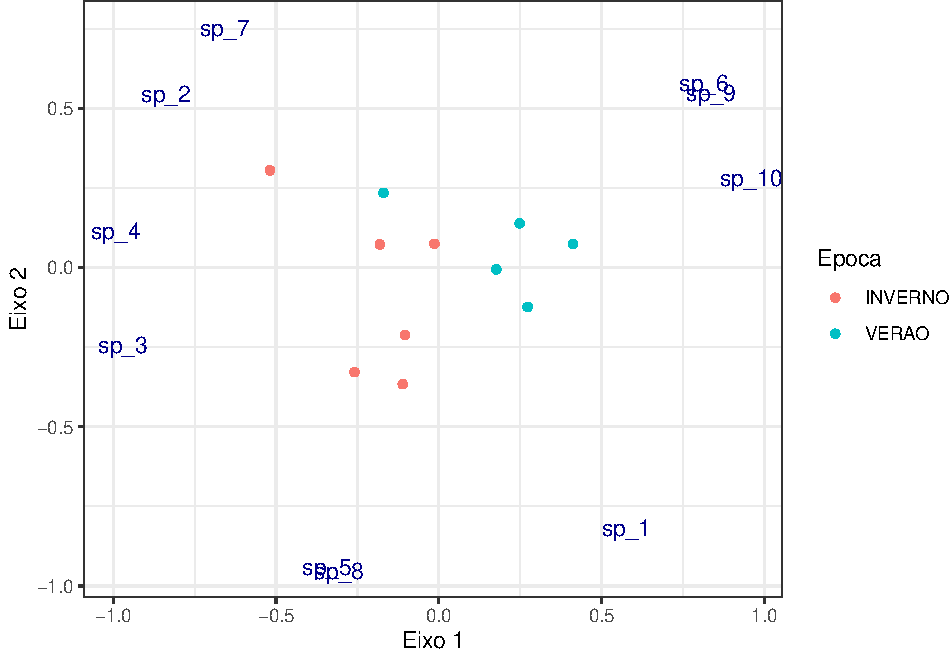
\includegraphics{medidas-diversidade_files/figure-latex/unnamed-chunk-41-1.pdf}

Temos acima um mapa com eixos \(1\) e \(2\). Cada ponto é uma amostra (temos 12 ao todo), identificadas de acordo com o período (INVERNO, VERAO). As espécies identificadas pelo seu nome.

A maior parte dos pontos do verão aparece na posição mais a direita, enquanto os pontos de inverno mais a esquerda. Isto sugere que as amostras com composições mais similares entre si tendem a ser amostras coletadas em um mesmo período.

Posicionar as espécies nos ajuda a saber quais delas tendem a ser mais frequentes em cada período. As espécies à direita tendem a ser mais frequêntes no verão e as espécies mais à esquerda no inverno. Compare esta figura com nossa matriz original.

\begin{Shaded}
\begin{Highlighting}[]
\NormalTok{pe }\SpecialCharTok{\%\textgreater{}\%} 
  \FunctionTok{select}\NormalTok{(Epoca}\SpecialCharTok{:}\NormalTok{sp\_10) }\SpecialCharTok{\%\textgreater{}\%} 
  \FunctionTok{View}\NormalTok{()}
\end{Highlighting}
\end{Shaded}

\begin{table}
\centering\begingroup\fontsize{10}{12}\selectfont

\begin{tabular}{l|r|r|r|r|r|r|r|r|r|r}
\hline
Epoca & sp\_1 & sp\_2 & sp\_3 & sp\_4 & sp\_5 & sp\_6 & sp\_7 & sp\_8 & sp\_9 & sp\_10\\
\hline
\cellcolor[HTML]{7be896}{\textcolor{black}{INVERNO}} & \cellcolor[HTML]{7be896}{\textcolor{black}{5}} & \cellcolor[HTML]{7be896}{\textcolor{black}{6}} & \cellcolor[HTML]{7be896}{\textcolor{black}{72}} & \cellcolor[HTML]{7be896}{\textcolor{black}{65}} & \cellcolor[HTML]{7be896}{\textcolor{black}{8}} & \cellcolor[HTML]{7be896}{\textcolor{black}{6}} & \cellcolor[HTML]{7be896}{\textcolor{black}{1}} & \cellcolor[HTML]{7be896}{\textcolor{black}{0}} & \cellcolor[HTML]{7be896}{\textcolor{black}{0}} & \cellcolor[HTML]{7be896}{\textcolor{black}{0}}\\
\hline
\cellcolor[HTML]{7be896}{\textcolor{black}{INVERNO}} & \cellcolor[HTML]{7be896}{\textcolor{black}{6}} & \cellcolor[HTML]{7be896}{\textcolor{black}{0}} & \cellcolor[HTML]{7be896}{\textcolor{black}{1}} & \cellcolor[HTML]{7be896}{\textcolor{black}{18}} & \cellcolor[HTML]{7be896}{\textcolor{black}{9}} & \cellcolor[HTML]{7be896}{\textcolor{black}{12}} & \cellcolor[HTML]{7be896}{\textcolor{black}{0}} & \cellcolor[HTML]{7be896}{\textcolor{black}{1}} & \cellcolor[HTML]{7be896}{\textcolor{black}{0}} & \cellcolor[HTML]{7be896}{\textcolor{black}{0}}\\
\hline
\cellcolor[HTML]{7be896}{\textcolor{black}{INVERNO}} & \cellcolor[HTML]{7be896}{\textcolor{black}{7}} & \cellcolor[HTML]{7be896}{\textcolor{black}{0}} & \cellcolor[HTML]{7be896}{\textcolor{black}{0}} & \cellcolor[HTML]{7be896}{\textcolor{black}{48}} & \cellcolor[HTML]{7be896}{\textcolor{black}{2}} & \cellcolor[HTML]{7be896}{\textcolor{black}{0}} & \cellcolor[HTML]{7be896}{\textcolor{black}{0}} & \cellcolor[HTML]{7be896}{\textcolor{black}{4}} & \cellcolor[HTML]{7be896}{\textcolor{black}{0}} & \cellcolor[HTML]{7be896}{\textcolor{black}{0}}\\
\hline
\cellcolor[HTML]{7be896}{\textcolor{black}{INVERNO}} & \cellcolor[HTML]{7be896}{\textcolor{black}{0}} & \cellcolor[HTML]{7be896}{\textcolor{black}{0}} & \cellcolor[HTML]{7be896}{\textcolor{black}{0}} & \cellcolor[HTML]{7be896}{\textcolor{black}{13}} & \cellcolor[HTML]{7be896}{\textcolor{black}{4}} & \cellcolor[HTML]{7be896}{\textcolor{black}{1}} & \cellcolor[HTML]{7be896}{\textcolor{black}{0}} & \cellcolor[HTML]{7be896}{\textcolor{black}{0}} & \cellcolor[HTML]{7be896}{\textcolor{black}{0}} & \cellcolor[HTML]{7be896}{\textcolor{black}{0}}\\
\hline
\cellcolor[HTML]{7be896}{\textcolor{black}{INVERNO}} & \cellcolor[HTML]{7be896}{\textcolor{black}{2}} & \cellcolor[HTML]{7be896}{\textcolor{black}{0}} & \cellcolor[HTML]{7be896}{\textcolor{black}{143}} & \cellcolor[HTML]{7be896}{\textcolor{black}{48}} & \cellcolor[HTML]{7be896}{\textcolor{black}{1}} & \cellcolor[HTML]{7be896}{\textcolor{black}{0}} & \cellcolor[HTML]{7be896}{\textcolor{black}{0}} & \cellcolor[HTML]{7be896}{\textcolor{black}{1}} & \cellcolor[HTML]{7be896}{\textcolor{black}{0}} & \cellcolor[HTML]{7be896}{\textcolor{black}{0}}\\
\hline
\cellcolor[HTML]{7be896}{\textcolor{black}{INVERNO}} & \cellcolor[HTML]{7be896}{\textcolor{black}{0}} & \cellcolor[HTML]{7be896}{\textcolor{black}{0}} & \cellcolor[HTML]{7be896}{\textcolor{black}{95}} & \cellcolor[HTML]{7be896}{\textcolor{black}{28}} & \cellcolor[HTML]{7be896}{\textcolor{black}{0}} & \cellcolor[HTML]{7be896}{\textcolor{black}{0}} & \cellcolor[HTML]{7be896}{\textcolor{black}{1}} & \cellcolor[HTML]{7be896}{\textcolor{black}{0}} & \cellcolor[HTML]{7be896}{\textcolor{black}{0}} & \cellcolor[HTML]{7be896}{\textcolor{black}{0}}\\
\hline
\cellcolor[HTML]{e8867b}{\textcolor{black}{VERAO}} & \cellcolor[HTML]{e8867b}{\textcolor{black}{1}} & \cellcolor[HTML]{e8867b}{\textcolor{black}{0}} & \cellcolor[HTML]{e8867b}{\textcolor{black}{0}} & \cellcolor[HTML]{e8867b}{\textcolor{black}{8}} & \cellcolor[HTML]{e8867b}{\textcolor{black}{0}} & \cellcolor[HTML]{e8867b}{\textcolor{black}{27}} & \cellcolor[HTML]{e8867b}{\textcolor{black}{0}} & \cellcolor[HTML]{e8867b}{\textcolor{black}{0}} & \cellcolor[HTML]{e8867b}{\textcolor{black}{1}} & \cellcolor[HTML]{e8867b}{\textcolor{black}{0}}\\
\hline
\cellcolor[HTML]{e8867b}{\textcolor{black}{VERAO}} & \cellcolor[HTML]{e8867b}{\textcolor{black}{0}} & \cellcolor[HTML]{e8867b}{\textcolor{black}{0}} & \cellcolor[HTML]{e8867b}{\textcolor{black}{0}} & \cellcolor[HTML]{e8867b}{\textcolor{black}{1}} & \cellcolor[HTML]{e8867b}{\textcolor{black}{3}} & \cellcolor[HTML]{e8867b}{\textcolor{black}{2}} & \cellcolor[HTML]{e8867b}{\textcolor{black}{2}} & \cellcolor[HTML]{e8867b}{\textcolor{black}{0}} & \cellcolor[HTML]{e8867b}{\textcolor{black}{0}} & \cellcolor[HTML]{e8867b}{\textcolor{black}{0}}\\
\hline
\cellcolor[HTML]{e8867b}{\textcolor{black}{VERAO}} & \cellcolor[HTML]{e8867b}{\textcolor{black}{8}} & \cellcolor[HTML]{e8867b}{\textcolor{black}{0}} & \cellcolor[HTML]{e8867b}{\textcolor{black}{0}} & \cellcolor[HTML]{e8867b}{\textcolor{black}{1}} & \cellcolor[HTML]{e8867b}{\textcolor{black}{4}} & \cellcolor[HTML]{e8867b}{\textcolor{black}{6}} & \cellcolor[HTML]{e8867b}{\textcolor{black}{0}} & \cellcolor[HTML]{e8867b}{\textcolor{black}{0}} & \cellcolor[HTML]{e8867b}{\textcolor{black}{4}} & \cellcolor[HTML]{e8867b}{\textcolor{black}{0}}\\
\hline
\cellcolor[HTML]{e8867b}{\textcolor{black}{VERAO}} & \cellcolor[HTML]{e8867b}{\textcolor{black}{2}} & \cellcolor[HTML]{e8867b}{\textcolor{black}{0}} & \cellcolor[HTML]{e8867b}{\textcolor{black}{0}} & \cellcolor[HTML]{e8867b}{\textcolor{black}{0}} & \cellcolor[HTML]{e8867b}{\textcolor{black}{6}} & \cellcolor[HTML]{e8867b}{\textcolor{black}{2}} & \cellcolor[HTML]{e8867b}{\textcolor{black}{0}} & \cellcolor[HTML]{e8867b}{\textcolor{black}{0}} & \cellcolor[HTML]{e8867b}{\textcolor{black}{0}} & \cellcolor[HTML]{e8867b}{\textcolor{black}{0}}\\
\hline
\cellcolor[HTML]{e8867b}{\textcolor{black}{VERAO}} & \cellcolor[HTML]{e8867b}{\textcolor{black}{1}} & \cellcolor[HTML]{e8867b}{\textcolor{black}{0}} & \cellcolor[HTML]{e8867b}{\textcolor{black}{0}} & \cellcolor[HTML]{e8867b}{\textcolor{black}{3}} & \cellcolor[HTML]{e8867b}{\textcolor{black}{0}} & \cellcolor[HTML]{e8867b}{\textcolor{black}{2}} & \cellcolor[HTML]{e8867b}{\textcolor{black}{0}} & \cellcolor[HTML]{e8867b}{\textcolor{black}{0}} & \cellcolor[HTML]{e8867b}{\textcolor{black}{1}} & \cellcolor[HTML]{e8867b}{\textcolor{black}{0}}\\
\hline
\cellcolor[HTML]{e8867b}{\textcolor{black}{VERAO}} & \cellcolor[HTML]{e8867b}{\textcolor{black}{1}} & \cellcolor[HTML]{e8867b}{\textcolor{black}{0}} & \cellcolor[HTML]{e8867b}{\textcolor{black}{0}} & \cellcolor[HTML]{e8867b}{\textcolor{black}{0}} & \cellcolor[HTML]{e8867b}{\textcolor{black}{0}} & \cellcolor[HTML]{e8867b}{\textcolor{black}{7}} & \cellcolor[HTML]{e8867b}{\textcolor{black}{0}} & \cellcolor[HTML]{e8867b}{\textcolor{black}{0}} & \cellcolor[HTML]{e8867b}{\textcolor{black}{0}} & \cellcolor[HTML]{e8867b}{\textcolor{black}{1}}\\
\hline
\end{tabular}
\endgroup{}
\end{table}

Veja que as especies sp\_9 e sp\_10 ocorrem somente no verão. A espécie sp\_6 ocorre em \textbf{todas} as amostras de verão, ainda que também esteja presente no inverno.

A sp\_3 por outro lado ocorre somente no inverno, aparacendo como a espécie mais a esquerda na figura.

Finalmente, a sp\_1 fica exatamente no meio do caminho, pois ocorre em \textbf{todas as 12 amostras}.

Utilizando este tipo de representação, podemos interpretar facilmente grandes matrizes de distância e compreender os padrões de variação (diversidade \(\beta\)) entre nossas amostras.

\hypertarget{salvando-as-figuras-deste-tutorial}{%
\section{Salvando as figuras deste tutorial}\label{salvando-as-figuras-deste-tutorial}}

Este tutorial utilizou a base de dados: Baia\_santos.xlsx como exemplo. Você pode replicá-lo para sua tabela de dados fazendo as devidas alterações de nomenclatura (ex. os nomes das colunas).

Após rodar estas funções geramos uma série de figuras. Estas figuras podem ser salvas no formato \textbf{.png} (outro outro tipo de imagem) utilizando os comandos:

\begin{Shaded}
\begin{Highlighting}[]
\NormalTok{div\_alfa }\OtherTok{=}\NormalTok{ plt\_D }\SpecialCharTok{|}\NormalTok{ plt\_S }\SpecialCharTok{|}\NormalTok{ plt\_E}
\FunctionTok{ggsave}\NormalTok{(}\AttributeTok{filename =} \StringTok{\textquotesingle{}Diversidade\_alfa.png\textquotesingle{}}\NormalTok{, }
       \AttributeTok{plot =}\NormalTok{ div\_alfa, }
       \AttributeTok{width =} \DecValTok{15}\NormalTok{, }\AttributeTok{height =} \DecValTok{5}\NormalTok{)}

\NormalTok{div\_gama }\OtherTok{=}\NormalTok{ plt\_gama}
\FunctionTok{ggsave}\NormalTok{(}\AttributeTok{filename =} \StringTok{\textquotesingle{}Diversidade\_gama.png\textquotesingle{}}\NormalTok{, }
       \AttributeTok{plot =}\NormalTok{ div\_gama, }
       \AttributeTok{width =} \DecValTok{7}\NormalTok{, }\AttributeTok{height =} \DecValTok{5}\NormalTok{)}

\NormalTok{div\_beta }\OtherTok{=}\NormalTok{ plt\_beta}
\FunctionTok{ggsave}\NormalTok{(}\AttributeTok{filename =} \StringTok{\textquotesingle{}Diversidade\_beta.png\textquotesingle{}}\NormalTok{, }
       \AttributeTok{plot =}\NormalTok{ div\_beta,}
       \AttributeTok{width =} \DecValTok{7}\NormalTok{, }\AttributeTok{height =} \DecValTok{5}\NormalTok{)}
\end{Highlighting}
\end{Shaded}

Após rodar estes comandos, as figuras serão salvas em sua pasta de trabalho, aquela que você definiu no início desta seção.

\hypertarget{videoaulas}{%
\chapter{Links para as vídeo-aulas e base de dados}\label{videoaulas}}

\begin{center}\rule{0.5\linewidth}{0.5pt}\end{center}

\begin{quote}
As vídeo aulas referentes ao conteúdo desta apostila podem ser encontradas abaixo:
\end{quote}

\begin{itemize}
\item
  Medidas de diversidade - 01 - Indice de diversidade
\item
  Medidas de diversidade - 02 - Diversidade na paisagem
\item
  Medidas de diversidade - 03 - Diversidade alfa
\item
  Medidas de diversidade - 04 - Diversidade gama
\item
  Medidas de diversidade - 05 - Diversidade beta
\item
  Medidas de diversidade - 06 - Tutorial no R
\end{itemize}

\begin{center}\rule{0.5\linewidth}{0.5pt}\end{center}

\begin{quote}
O tutorial rápido em \textbf{pdf} e a base com os dados utilizados no exemplo podem ser acessados em:
\end{quote}

\begin{itemize}
\item
  Tutorial em R - Medidas e Escalas de diversidade
\item
  Baia\_santos.xlsx
\end{itemize}

\begin{center}\rule{0.5\linewidth}{0.5pt}\end{center}

  \bibliography{book.bib,packages.bib}

\end{document}
